\minitoc
\begin{refsection}
\newpage
\fbox{\begin{minipage}{\textwidth}
    \textbf{Contexte :}\\
    Dans l'article \cite{ribeyre_2016}, un modèle a été développé pour estimer le nombre de paires produites dans la collision de deux faisceaux de photons. Ce modèle prend en compte la divergence des sources et leur distance de collision, mais pas la taille initiale des sources ou leur durées, ni l'angle de collision entre les faisceaux ou la distribution en énergie des photons. Deux autres articles \parencite{ribeyre_2017, ribeyre_2018} ont aussi étudié la cinématique des paires produites dans la collision de deux photons, et ne prenaient donc pas en compte la distribution en énergie des faisceaux de photons incidents.

    \medskip
    \textbf{Résumé du chapitre :}\\
    Dans ce chapitre, des développements théoriques permettant d'estimer le nombre et les caractéristiques cinématiques de paires produites dans la collision de deux faisceaux de photons avec des distributions en énergies larges sont présentés. Le nombre de paires peut être exprimé comme le produit de la luminosité simple collision, qui prend en compte les aspects géométriques de la collision, par une section efficace intégrée, qui prend en compte ses aspects énergétiques (équation (\ref{eq:51-N+_definition})). Une estimation de la luminosité simple collision est dérivée en considérant l'interaction de deux pavés de densités constantes, avec un angle de collision variable (équation (\ref{eq:52-luminosite_pinceaux}). Cette quantité est maximisée pour la collision de sources de photons avec l'extension spatio-temporelle la plus faible possible. La diminution de la luminosité induite par une désynchronisation des faisceaux, par un paramètre d'impact non nul, ou par l'effet de la divergence des photons, est ensuite calculée (équations (\ref{eq:52-luminosite_desynchro}), (\ref{eq:52-luminosite_parametre_impact}) et (\ref{eq:52-luminosite_divergence}) respectivement). Il est montré que les sources d'extension spatio-temporelle importantes telles que les sources Bremsstrahlung sont assez peu sensibles à ces variations de conditions expérimentales. Sous certaines conditions, il est aussi possible de montrer que la section efficace intégrée se réduit à une fonction d'une seule variable (équation (\ref{eq:53-sigma_int_s_eta})). Une paramétrisation de sources de type Compton inverse linéaire, Compton inverse multi-photon et Bremsstrahlung est ensuite effectuée (tableau \ref{tab:53-g_definitions}), et la section efficace intégrée correspondante est calculée numériquement. Il est montré que les sources Compton inverse linéaire et Bremsstrahlung optimales présentent des caractéristiques énergétiques déjà disponibles en laboratoire, et que celles-ci sont assez efficaces pour la création de paires par BWL. En dépit de leurs caractéristiques a priori moins intéressantes, les sources Compton inverse multi-photon produites par un laser dans un micro-canal pourraient néanmoins permettre de produire un grand nombre de paires, grâce à leur important nombre de photons, leur faible extension spatio-temporelle et leur faible divergence. Les données obtenues numériquement peuvent être reproduites avec une bonne précision grâce à la fonction d'ajustement dont les paramètres sont donnés dans le tableau \ref{tab:53-h_fit}. Ce chapitre se termine ensuite par la présentation d'un autre modèle permettant d'estimer les caractéristiques des positrons créés dans la collision de deux faisceaux de photons, produits par les processus Compton inverse multi-photon et Bremsstrahlung. Dans ce modèle, la distributions en énergie de chaque faisceau est approximée par une distribution de Dirac, et les caractéristiques des positrons produits sont estimées à l'aide d'un modèle de cinématique relativiste déjà publié \parencite{ribeyre_2017}. 
    
    \medskip
    \textbf{Informations complémentaires :}\\
    Plus d'informations sur la notion de luminosité sont disponibles dans l'article de \cite{herr_2006}, tandis que des détails sur le calcul de la section efficace intégrée sont aussi décrits dans une publication qui a été soumise à la revue \textit{New Journal of Physics} \parencite{esnault_2021}. Le modèle de cinématique relativiste est expliqué plus en détail au chapitre \ref{chap:1-particules} et dans la référence \parencite{ribeyre_2017}.
\end{minipage}}
\newpage

\section{Principe du modèle}

Dans cette section, nous dériverons une estimation du \textbf{nombre de positrons} qui pourraient être produits par la collision de deux faisceaux de photons avec une \textbf{distribution en énergie large}. Cette estimation reposera sur une adaptation du formalisme de la \textbf{luminosité} \parencite{herr_2006}, qui est très utilisé pour estimer l'occurrence de divers processus dans les collision de faisceaux de particules chargées dans les collisionneurs de particules. Nous verrons que, sous certaines hypothèses, il nous sera possible de séparer les propriétés géométriques des sources de photons (taille typique, durée, distance de collision …) de leurs propriétés énergétiques. Nous supposerons que les faisceaux de photons ont une \textbf{divergence nulle}, même si l'effet d'une divergence non-nulle sera estimée dans la section suivante. La dérivation de ce modèle (première section de ce chapitre) ainsi que la discussion concernant l'effet de la distribution en énergie sur le nombre de paires produites (troisième section de ce chapitre) sont décrits dans une publication qui a été soumise à la revue \textit{New Journal of Physics} \parencite{esnault_2021}.

Dans la collision de deux faisceaux de photons sans divergence, tel qu'illustré en figure \ref{fig:51-collision_faisceaux}, le taux de production volumique de paires électron-positron par le processus Breit-Wheeler linéaire peut être estimé via l'expression \parencite{gould_1971, landau_1975} :
\begin{equation}
    \dfrac{d n_+}{dt} = \iint c ~ (1-\cos{\psi_{12}}) ~ \dfrac{d n_1}{d E_1} ~ \dfrac{d n_2}{d E_2} ~ \sigma_{\gamma\gamma} ~ d E_1 ~ d E_2 ~ \rm ,
    \label{eq:51-taux_positrons}
\end{equation}

avec $n_+$ la densité volumique de positrons, $dt$ un temps infinitésimal, $c$ la vitesse de la lumière dans le vide, $\psi_{12}$ l'angle de collision entre les deux faisceaux, $n_i$ la densité volumique de photons (en nombre par unité de volume) du faisceau $i$ ($i=\{1,2\}$), $E_i$ l'énergie des photons du faisceau $i$ et $\sigma_{\gamma\gamma}$ la section efficace Breit-Wheeler linéaire définie par \parencite{greiner_2009} :
\begin{equation}
\begin{split}
    \sigma_{\gamma\gamma}(s)= 4 \pi r_e^2 \frac{m_e^2 c^4}{s} \Bigg[ \left(2 + \frac{8 m_e^2 c^4}{s} - \frac{16 m_e^4 c^8}{s^2}\right) \ln \frac{\sqrt{s} + \sqrt{s - 4 m_e^2 c^4}}{2 m_e c^2} \\
    - \sqrt{1 - \frac{4 m_e^2 c^4}{s}}\left(1 + 4 \frac{m_e^2 c^4}{s}\right)\Bigg]
\end{split}
\label{eq:51-sigma_BWL}
\end{equation}
avec $r_e = e^2/4 \pi \varepsilon_0  m_e c^2 \approx 2.8 \times 10^{-13} ~ \si{\cm}$ le rayon classique de l'électron, $m_e$ la masse de l'électron, et $s$ la variable de Mandelstam de masse invariante au carré définie comme $s=2 E_1 E_2 (1-\cos{\psi_{12}}) = E_{CM}^2$, avec $E_{CM}$ l'énergie du centre d'inertie du système. Pour des faisceaux de photons sans divergence, les particules de chaque faisceau sont parallèles entre elles. Ainsi, seuls les photons de faisceaux différents peuvent collisionner ensemble, et l'angle de collision entre ces photons est identique à l'angle de collision entre les faisceaux $\psi_{12}$.

Comme nous l'avons vu au chapitre \ref{chap:1-particules}, la section efficace BWL donnée par l'équation (\ref{eq:51-sigma_BWL}) et représentée en figure \ref{fig:51-sigma_BWL} dépend d'un seul paramètre $s$, et a un seuil de production de paires pour $\sqrt{s}=2 m_e c^2$. Son maximum est situé autour de $\sqrt{s} \approx 1.43 ~ \si{\MeV}$, et son amplitude maximale est divisée par 10 pour une valeur de $\sqrt{s} \approx 8.47$ MeV.

\begin{figure}[t]
    \begin{minipage}[b]{0.4\linewidth}
    	\centering
    	\includegraphics[width=\linewidth]{5-opti_theorique/beam-beam_collision.png}
    	\caption{Illustration de la collision de deux faisceaux de photons sans divergence. Les deux faisceaux collisionnent avec un angle $\psi_{12}$ et produisent des paires électron-positron, représenté par les nuages bleu et rouge.}
    	\label{fig:51-collision_faisceaux}
    \end{minipage}
    \hfill
    \begin{minipage}[b]{0.5\linewidth}
    	\centering
    	\includegraphics[width=\linewidth]{5-opti_theorique/LBW_cross_section.png}
    	\caption{Section efficace Breit-Wheeler linéaire, en $r_e^2$, en fonction de l'énergie du centre d'inertie $\sqrt{s}=E_{CM}$ en MeV.}
    	\label{fig:51-sigma_BWL}
    \end{minipage}
\end{figure}

Pour estimer le nombre total de positrons $N_+$ (ou de manière équivalente le nombre total d'électrons) produits par le processus BWL dans la collision de ces deux faisceaux, il nous suffit alors d'intégrer le taux de production volumique de positrons donné par l'équation (\ref{eq:51-taux_positrons}) sur tout le volume d'interaction pendant toute sa durée, soit :
\begin{equation}
N_+ = \iiiint \dfrac{d n_+}{dt} ~ d^3V ~ dt ~ .
\end{equation}

On considère ensuite ici que les sources de photons ont une \textbf{distribution en énergie} qui est \textbf{indépendante de la position} considérée dans le faisceau, i.e. que l'on peut écrire la densité volumique de photons $n_i$ comme le produit d'un terme spatio-temporel avec un terme énergétique :
\begin{equation}
    \dfrac{dn_i(\textbf{x}, t, E_i)}{dE_i} = N_i \times \rho_i (\textbf{x}, t) \times f_i (E_i) ~ \rm ,
\end{equation}

avec $\textbf{x}$ le vecteur position, $N_i$ le nombre total de photons dans le faisceau $i$, $\rho_i$ leur densité volumique normalisée (dont l'intégrale sur tout l'espace vaut $1$), et $f_i$ une fonction de distribution en énergie (FDE), où $f_i(E_i)$ est la probabilité d'obtenir un photon d'énergie comprise entre $E_i$ et $E_i+dE_i$.

Sous cette condition, nous pouvons séparer cette intégrale et exprimer le \textbf{nombre total de paires produites} $N_+$ comme le \textbf{produit de deux termes} :
\begin{equation}
    N_+ = \mathcal{L}_{12}^{sc} \times \sigma_{\gamma\gamma}^{int} ~ \rm ,
    \label{eq:51-N+_definition}
\end{equation}

où $\mathcal{L}_{12}^{sc}$ est la \textit{luminosité simple collision} (cette appellation sera explicitée dans la section suivante) \parencite{herr_2006}, définie comme :
\begin{equation}
    \mathcal{L}_{12}^{sc} = c ~ (1-\cos{\psi_{12}}) ~ N_1 ~ N_2 \iiiint_{-\infty}^{+\infty} \rho_1 ~ \rho_2 ~ d^3 V ~ dt
    \label{eq:51-luminosite_definition}
\end{equation}
et où $\sigma_{\gamma\gamma}^{int}$ est appelée \textit{section efficace intégrée}. Cette quantité prend en compte les aspects énergétiques dans la collision des deux faisceaux, et est définie par :
\begin{equation}
    \sigma_{\gamma\gamma}^{int} = \iint_{0}^{+\infty} f_1 ~ f_2 ~ \sigma_{\gamma\gamma} ~ dE_1 ~ dE_2.
    \label{eq:51-sigma_int_definition}
\end{equation}

Chacune de ces deux quantités peut alors permettre d'apporter un éclairage spécifique sur le problème de l'optimisation du nombre de positrons $N_+$.

La \textbf{luminosité simple collision} $\mathcal{L}_{12}^{sc}$ ne dépend en effet que de \textbf{facteurs géométriques}, et est donc fortement dépendante des mécanismes de productions des photons et des conditions expérimentales. Nous pouvons néanmoins déjà mentionner que cette quantité, de dimension homogène à l'inverse d'une surface, sera a priori maximisée \textbf{pour un angle de collision $\psi_{12} \sim 180$ degrés}, et que le nombre de paires produites est proportionnel au \textbf{produit du nombre de photons de chaque source}. 

De l'autre côté, la section efficace intégrée $\sigma_{\gamma\gamma}^{int}$ ne dépend pas des propriétés spatio-temporelles des sources mais seulement des \textbf{distributions en énergies} des faisceaux de photons, pour un angle de collision donné. Pour un couple $f_1$, $f_2$ de distributions en énergies donné, elle peut être calculée \textbf{une fois pour toutes}, et sa maximisation peut permettre \textbf{d'optimiser les paramètres énergétiques des sources de photons} pour maximiser le nombre de paires $e^-e^+$ produites.

Il est intéressant de noter que l'intégrale permettant de calculer de $\sigma_{\gamma\gamma}^{int}$ est très similaire au calcul de sections efficaces faisant intervenir des photons virtuels sous la double approximation de photon équivalents \parencite{greiner_2009, kessler_1974}, où les fonctions $f_i$ sont remplacées par les spectres équivalents de photons virtuels. Cette méthode permet notamment de calculer la production de paires dans la diffusion de particules chargées, processus appelé Landau-Lifshitz, et qui sous la double approximation de photon équivalent s'interprète comme la collision de deux photons virtuels créant une paire électron-positron (voir chapitre \ref{chap:1-particules}). Pour obtenir une formulation analytique de cette section efficace, il est notamment nécessaire de considérer la limite ultra-relativiste de $\sigma_{\gamma\gamma}$ \parencite{greiner_2009}, ce qui n'est cependant pas notre cas ici. 

Dans la suite de ce chapitre, nous verrons tout d'abord comment calculer la luminosité géométrique de faisceaux de formes très simples, ce qui nous permettra de déterminer les paramètres clés pour la maximisation du nombre de paires produites. Nous pourrons ensuite utiliser ces formules pour tenter d'estimer la dépendance du nombre de paires à des variations de conditions expérimentales, telles que la variation de l'angle de collision ou encore l'effet d'un mauvais alignement ou d'une désynchronisation des faisceaux de photons par exemple. 

Nous calculerons ensuite quelques sections efficaces intégrées en considérant des distributions en énergies de photons assez simples. Nous nous intéresserons en particulier à trois formes de distributions en énergies, permettant de modéliser les sources de photons produites par Bremsstrahlung, Compton inverse linéaire et Compton inverse multi-photon. Ces résultats nous aiderons à déterminer quels types de distribution en énergies seraient les plus efficaces pour la création de paires par le processus BWL, en maximisant le nombre de paires produites. Les calculs développés pour cette section sont aussi adaptables à d'autres types de distribution en énergie, voire à l'étude d'autres processus de collision de particules.

Enfin, nous présenterons un autre modèle permettant d'estimer rapidement la distribution en énergie et en angle des positrons produits par de telles sources de photons. Ce chapitre sera clôturé par une estimation des principales caractéristiques des positrons produits lors de la collision de deux sources de type Bremsstrahlung, pour différents angles de collision.

Pour l'estimation du nombre total de paires produites dans la collision de deux faisceaux de photons, le modèle de \cite{ribeyre_2016} permet déjà d'estimer l'influence de la divergence des faisceaux, de leur distance de collision, et de l'énergie totale contenue dans les faisceaux de photons. Les aspects liés à une variation d'angle de collision, à l'extension spatio-temporelle des faisceaux de photons (taille typique et durée) ne sont néanmoins pas considérés, et ce modèle ne permet pas non plus de déterminer quelles formes de distributions en énergies sont les plus efficaces pour la création de paires.
Le modèle développé dans la suite de ce chapitre nous permettra quant à lui d'estimer l'influence de ces paramètres sur le nombre de paires produites, et a de plus l'avantage de reposer sur un formalisme déjà bien connu (principalement dans la communauté des collisionneurs de particules \parencite{herr_2006}). Le second modèle présenté à la fin de ce chapitre permet de prendre en compte les aspects les plus importants de la distribution en énergie des photons, en se basant largement sur les résultats obtenus par \cite{ribeyre_2017}.

\section{Estimation de la luminosité géométrique}

Comme nous venons de l'évoquer, la luminosité géométrique, ou tout simplement luminosité, est un paramètre crucial pour l'optimisation de la production de paires électron-positron par collision de faisceaux de photons. Dans cette section, nous développerons un modèle simple pour estimer la dépendance de cette quantité à divers paramètres expérimentaux.

\subsection{Remarques générales}

La \textbf{luminosité simple collision}, dont la définition a été dérivée dans la section précédente, a donc la \textbf{dimension inverse de celle d'une surface}, qui peut être vue comme une \textbf{surface équivalente} lors de la collision des deux faisceaux. Dans le cas de particules massives, on peut se représenter la luminosité simple collision comme le flux d'un faisceau vu depuis le référentiel de l'autre faisceau, intégré sur le temps de collision total. Elle se calcule comme le produit d'un terme cinématique (qui vaut $c (1 -\cos{\psi_{12}})$ pour deux faisceaux de photons \parencite{gould_1971}) par l'intégrale spatio-temporelle des densités de photons \parencite{herr_2006}. Cette intégrale est en général difficile à calculer analytiquement \parencite{meshkov_2018} ; en particulier pour des collisions de particules chargées interagissant entre elles ou avec des champs externes \parencite{herr_2006}. Il est néanmoins possible sous certaines hypothèses d'en obtenir une formulation analytique, de l'estimer à l'aide de codes de calculs voire de la mesurer expérimentalement \parencite{herr_2006}.

Si on multiplie la luminosité simple collision par le taux de répétition de la machine (collisionneur de particules ou système laser), on obtient une quantité souvent appelée \textbf{luminosité} dans la communauté des collisionneurs de particules \parencite{herr_2006}. Elle permet d'estimer le nombre d’occurrences d'un processus \textbf{par seconde} dans une machine donnée, et ainsi de comparer les performances de différentes machines entre elles. La luminosité à donc une \textbf{croissance linéaire avec le taux de répétition}, et une \textbf{croissance quadratique avec le nombre de particules incidentes}.

Enfin, en multipliant cette dernière quantité par le temps total de l'expérience, il est aussi possible d'estimer le \textbf{nombre total d’occurrences d'un processus sur toute une campagne expérimentale}. On appelle cette quantité la \textbf{luminosité intégrée}, et elle permet d'estimer rapidement si un processus de section efficace donnée est susceptible d'être observé dans une machine donnée en un temps d'expérience raisonnable. 

Dans le cadre de cette thèse, et à titre d'exemple, nous développerons dans la suite un modèle très simple de collision de deux faisceaux \textbf{homogènes}. Celui-ci sera \textbf{peu précis} pour l'estimation \textbf{quantitative} du nombre de paires produites par des \textbf{sources de photons réalistes}, mais il nous permettra de développer une \textbf{compréhension intuitive} de l'effet des différents paramètres géométriques des faisceaux de photons (durée, rayon typique, divergence, …) sur le nombre de paires produites. Il nous permettra de plus d'estimer l'effet de l'angle de collision, d'un défaut d'alignement spatial ou de synchronisation entre les sources sur la production de paires. Cette étude pourra alors être utile au dimensionnement d'une expérience de collision de photons, et servir d'\textbf{estimations rapides d'ordres de grandeur}. 

Des formulations plus précises de la luminosité sont disponibles dans la littérature. Notamment, pour deux faisceaux gaussiens identiques contra-propagatifs (i.e. collisionnant avec angle de collision $\psi_{12}=180$ degrés), la luminosité simple collision s'écrit \parencite{herr_2006} :
\begin{equation}
    \mathcal{L}^{sc} = \dfrac{2 \ln(2) ~ N_1 N_2}{\pi D_t^2} ~ \rm ,
    \label{eq:52-luminosite_gaussien}
\end{equation}

avec $D_t$ la largeur à mi-hauteur de la densité de particules dans la direction transverse à la propagation des faisceaux.

D'autres formulations permettent de prendre en compte l'effet d'un angle de collision entre les faisceaux \parencite{hirata_1995}, de considérer des faisceaux de tailles différentes \parencite{meshkov_2018}, des distributions spatiales non gaussiennes ou encore des effets d'interactions électromagnétiques entre les particules chargées \parencite{herr_2006} … et celles-ci amènent généralement à une réduction de la luminosité définie dans l'équation (\ref{eq:52-luminosite_gaussien}). Néanmoins, ces formulations ne prennent en général pas en compte tous ces aspects simultanément \parencite{meshkov_2018}.

\subsection{Collision de deux pinceaux de densités constante}

Nous considérons donc ici le cas académique de la collision de deux faisceaux \textbf{parfaitement collimatés}, de forme \textbf{parallélépipédiques} de \textbf{section carrée} se propageant à la vitesse $c$. La densité de photons est supposée \textbf{homogène à l'intérieur} de ces pavés, et \textbf{nulle à l'extérieur}. Le schéma de cette collision est illustré en deux dimensions en figure \ref{fig:52-luminosite_collisions}a. Les flèches colorées indiquent la direction de propagation des faisceaux, et l'évolution temporelle est orientée de haut en bas. Le volume commun aux deux faisceaux est représenté en rouge. Nous cherchons alors à calculer la luminosité simple collision de ce type de géométrie, en estimant la valeur de l'intégrale définie par l'équation (\ref{eq:51-luminosite_definition}) :
\begin{equation*}
\mathcal{L}_{12}^{sc} = c ~ (1-\cos{\psi_{12}}) ~ N_1 ~ N_2 \iiiint_{-\infty}^{+\infty} \rho_1 ~ \rho_2 ~ d^3 V ~ dt ~ \rm ,
\end{equation*}

où nous rappelons que $\rho_i$ est la densité de photons normalisée du faisceau de photon $i$.

Dans la collision de ces deux faisceaux, nous pouvons distinguer trois phases :
\begin{itemize}
    \item  Une phase où les deux faisceaux se rencontrent, et où le \textbf{volume commun} à ces deux faisceaux \textbf{augmente avec le temps}. Cette phase est notée phase \textit{I} sur la figure \ref{fig:52-luminosite_collisions}a.
    
    \item Une phase où les faisceaux continuent de se propager, et où le \textbf{volume commun} aux deux faisceaux est \textbf{constant avec le temps}. Cette phase est notée phase \textit{II} sur la figure \ref{fig:52-luminosite_collisions}a.

    \item Une phase où les faisceaux se séparent, et où le \textbf{volume commun} aux deux faisceaux \textbf{diminue avec le temps}, jusqu'à devenir nul. Cette phase est notée phase \textit{III} sur la figure \ref{fig:52-luminosite_collisions}a.
\end{itemize}

Ainsi, dans les phases \textit{I} et \textit{III} le volume commun aux deux faisceaux évolue avec le temps, et celles-ci seront appelées les \textit{phases transitoires}. La phase \textit{II} sera quant à elle appelée \textit{phase pseudo-stationnaire}.

\begin{figure}[hbtp]
	\centering
	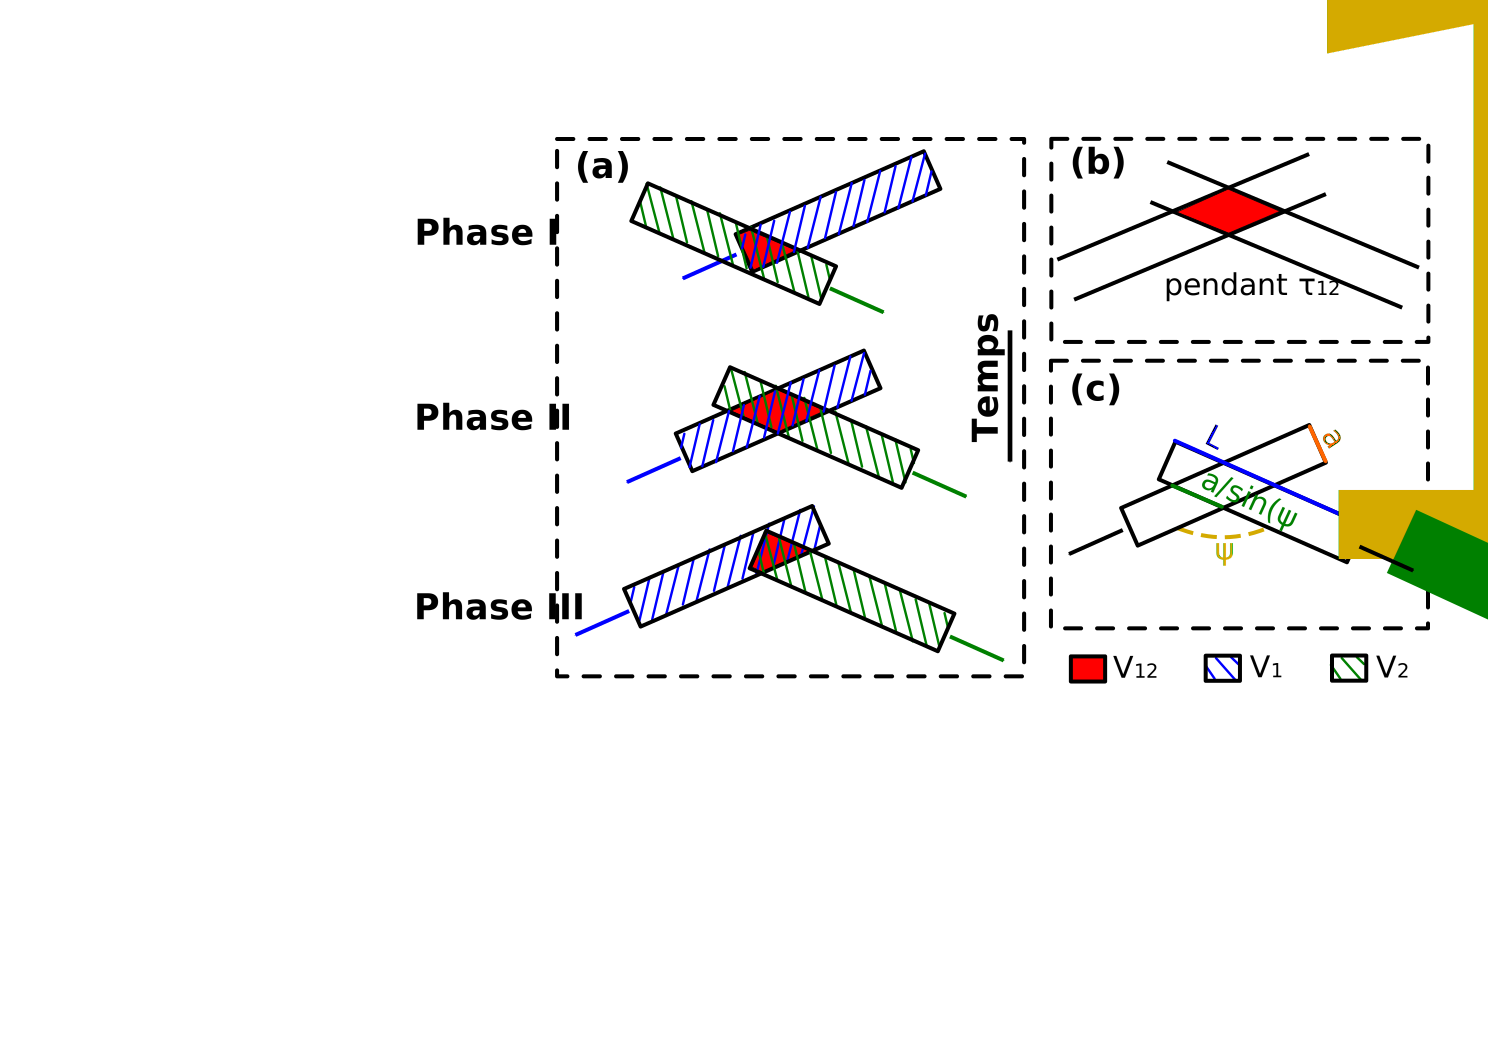
\includegraphics[width=\linewidth]{5-opti_theorique/collision_faisceaux.png}
	\caption{Illustrations de la collision de deux pavés de photons de densité homogènes. En (a) l'évolution temporelle du volume d'interaction est représentée, et est approximée en (b) par un volume d'interaction constant pendant un temps $\tau_{12}$. La définition des longueurs et angles est indiquée en (c).}
	\label{fig:52-luminosite_collisions}
\end{figure}

Pour des faisceaux de densités constantes, la densité normalisée $\rho_i$ du faisceau $i$ est :
\begin{equation}
    \rho_i =\left\{\begin{array}{@{}ll@{}} 1/V_i & \text{à l'intérieur du faisceau} \\0 & \text{a l'extérieur.}\end{array}\right.
\end{equation}

Dans ce cas, l'intégrale de l'équation (\ref{eq:51-luminosite_definition}) peut être calculée comme :
\begin{equation}
    \iiiint_{-\infty}^{+\infty} \rho_1 ~ \rho_2 ~ d^3 V dt= \int_{-\infty}^{+\infty}\dfrac{V_{12}(t)}{V_1 ~ V_2} ~ dt~ \rm ,
\end{equation}

où $V_{12}(t)$ est le volume commun aux deux faisceaux, évoluant avec le temps. 


Nous supposons dans un premier temps que ces faisceaux sont identiques, parfaitement synchronisés et alignés, et que leur taille transverse typique, notée $a$, est faible devant leur longueur, notée $L$. Ces faisceaux seront ici appelés \textit{pinceaux}. La définition de ces quantités est illustrée en figure \ref{fig:52-luminosite_collisions}c. Sous ces conditions, nous \textbf{négligeons} alors \textbf{l'influence de la phase transitoire devant la phase pseudo-stationnaire}. Nous considérons donc que le volume commun aux deux faisceaux $V_{12}$ est constant avec le temps pendant un temps $\tau_{12}$, et nul pour $t \notin [-\tau_{12}/2, \tau_{12}/2]$. Cette hypothèse est illustrée en figure \ref{fig:52-luminosite_collisions}b, et reviens à considérer la collision de faisceaux de longueur infinie pendant un temps fini. Dans ce cas, la luminosité simple collision peut donc être estimée comme :
\begin{equation}
    \mathcal{L}_{12}^{sc} \sim c ~ (1-\cos{\psi_{12}}) ~ N_1 ~ N_2 \times \tau_{12} \times \dfrac{V_{12}}{V_1 ~ V_2} ~ \rm .
\end{equation}

Pour la collision de deux pavés, le volume d'intersection $V_{12}$ est le produit de la surface commune aux deux faisceaux dans un plan donné, représentée par exemple en figure \ref{fig:52-luminosite_collisions}b, par leur hauteur commune, dans la direction transverse au plan de la figure \ref{fig:52-luminosite_collisions}b. Pour deux faisceaux parfaitement alignés, de section carrée d’arête $a$, et pour tout $\psi_{12}\neq 0^\circ$ et $\psi_{12}\neq 180^\circ$, ce volume d'intersection est donc :
\begin{equation}
    V_{12} = \dfrac{a^3}{\sin\psi_{12}} ~ \rm ,
\end{equation}

tandis que le volume de chaque pinceau est donné par :
\begin{equation}
V_i = a^2 L ~ \rm ;
\end{equation}

nous permettant d'exprimer la luminosité comme :
\begin{equation}
    \mathcal{L}_{12}^{sc} \sim \dfrac{N_1 ~ N_2 ~ c ~ \tau_{12}}{a L^2} \times \dfrac{(1-\cos{\psi_{12}})}{\sin{\psi_{12}}} ~ \rm .
    \label{eq:52-luminosite_temps}
\end{equation}

Puisque ces pinceaux sont identiques et parfaitement synchronisés, le temps total de collision est aussi de l'ordre de $\tau_{12} \sim L/c$, et la luminosité simple collision peut finalement s'écrire :
\begin{equation}
    \mathcal{L}_{12}^{sc} \sim \dfrac{N_1 ~ N_2}{a ~ c ~ \tau_{12}} \times \dfrac{(1-\cos{\psi_{12}})}{\sin{\psi_{12}}}\rm .
    \label{eq:52-luminosite_pinceaux}
\end{equation}

Comme cela a déjà été évoqué précédemment, le \textbf{nombre de paires} électron-positron produites dans la collision de deux faisceaux de photons est alors proportionnelle au \textbf{produit du nombre de photons de chaque faisceau}, soit une \textbf{dépendance quadratique au nombre de photons} pour des faisceaux identiques, et pour une section efficace considérée constante. La formulation de l'équation (\ref{eq:52-luminosite_pinceaux}) nous indique aussi que, sous ces conditions, la luminosité a une dépendance inverse à la taille transverse typique de ces sources, ainsi qu'une dépendance inverse à leur durée typique. Il semble alors que les sources de photons ayant la \textbf{densité de photon la plus importante} seront a priori les \textbf{plus efficaces pour la production de paires électron-positron}. Il est néanmoins intéressant de noter que, dans ce cadre, les propriétés spatio-temporelles des sources et le nombre total de photons ont un rôle aussi importants l'un que l'autre, et que les sources contenant un très grand nombre de photons ne seront pas forcement les plus efficaces si leur extension spatio-temporelle est trop importante. Enfin, nous pouvons aussi tracer la dépendance angulaire de la luminosité en figure \ref{fig:52-angle_luminosite}.

\begin{figure}[hbtp]
	\centering
	\includegraphics[width=0.7\linewidth]{5-opti_theorique/angle_luminosite.png}
	\caption{Dépendance de la luminosité à l'angle de collision, pour la collision de deux pinceaux de densités constantes.}
	\label{fig:52-angle_luminosite}
\end{figure}

Sur cette figure, nous pouvons remarquer que l'effet d'une variation de l'angle de collision semble très important pour des faibles valeurs ou des fortes valeurs de $\psi_{12}$, mais est plus limité pour des angles de collision s'approchant de 90 degrés. En prenant cet angle de collision pour référence, la valeur de la luminosité est divisée par 2 pour un angle de l'ordre de $53$ degrés, et est multipliée par 2 pour un angle autour de $127$ degrés. Pour des faibles angles de collision, la diminution de la luminosité se comprend comme étant une conséquence d'un plus faible nombre de collisions entre les photons. Ainsi, même en considérant des faisceaux de photons dont l'énergie est suffisante pour produire des paires (i.e. même si la condition $s=2 E_1 E_2 (1-\cos{\psi_{12}})>2m_e c^2$ est vérifiée), un \textbf{angle de collision faible} impliquera toujours une \textbf{diminution du nombre de paires produites}, à section efficace constante. Dans le cas limite $\psi_{12}=0$ degrés, aucune paire ne peux être produite puisque tous les photons se propagent parallèlement. Au contraire, la luminosité semble diverger pour un angle de collision $\psi_{12} \to 180$ degrés. Ce comportement est en fait une conséquence non physique des hypothèses de notre modèle, qui considère que le temps passé dans les phases transitoires est négligeable comparé au temps passé en phase pseudo-stationnaire. Cette hypothèse est alors non valide pour des faisceaux contra-propagatifs, où le volume commun au deux faisceaux n'est jamais constant avec le temps. 

Plus quantitativement, on peut estimer la durée de la phase transitoire en considérant 2 fois le temps que met un photon du faisceau 1 à traverser le faisceau 2 :
\begin{equation}
    \tau_{transi} \sim \dfrac{2}{c}\dfrac{a}{\sin\psi_{12}} ~ \rm ,
\end{equation}

où le facteur 2 permet de prendre en compte à la fois la phase \textit{I} et la phase \textit{III} de la figure \ref{fig:52-luminosite_collisions}a. La durée de la phase pseudo-stationnaire peut quant à elle être estimée comme étant de la durée totale des pinceaux (considérés identiques), à laquelle on a retranché la durée de la phase transitoire :
\begin{equation}
    \tau_{statio} \sim \dfrac{L}{c} -\tau_{transi} ~ \rm .
\end{equation}

L'angle de collision $\psi_{12}^{lim}$ à partir duquel $\tau_{transi}\sim \tau_{statio}/10$ est donc donné par :
\begin{equation}
    \sin{\psi_{12}^{lim}} \sim \dfrac{22 a}{L} ~ \rm ,
\end{equation}

et vaut environ 13° ou 167° pour $a/L \sim 1/100$. Cette hypothèse est donc très restrictive, car elle nécessite des faisceaux extrêmement fins et longs pour être valide pour des angles proches de 0 ou 180 degrés. Pour des faisceaux de dimensions données, notre hypothèse est la mieux vérifiée pour des angles collisions proches de 90 degrés, où le temps de la phase transitoire est le plus faible devant la phase pseudo-stationnaire. Nous savons néanmoins que la luminosité doit être nulle pour $\psi_{12} \sim 0^\circ$, car la collision de particules parallèles n'est pas possibles. Elle doit aussi être maximisée pour $\psi_{12} \sim 180^\circ$, car ce cas maximise le nombre de collision entre deux faisceaux \parencite{herr_2006}. Pour la collision de deux pavés identiques de section carrées d’arête $a$ parfaitement alignés, la luminosité simple collision à un angle de collision de 180 degrés s'écrit par ailleurs simplement :
\begin{equation}
    \mathcal{L}_{12}^{sc}(\psi_{12}=180^\circ) = \dfrac{N_1 N_2}{a^2} ~ \rm ,
    \label{eq:52-luminosite_contre_propagatif}
\end{equation}

et cette valeur constitue une limite théorique maximale à $\mathcal{L}_{12}^{sc}$.

\subsection{Dépendance de la luminosité à des variations de conditions expérimentales}

Dans le cas précédent, nous avons considéré des pinceaux identiques, parfaitement synchronisés, parfaitement alignés et parfaitement collimatés. Néanmoins, notre modèle simple de collisions de pavés peut aussi nous permettre d'estimer facilement l'influence de variations de conditions expérimentales, tels qu'une mauvaise synchronisation ou un mauvais alignement entre les faisceaux par exemple.

En effet, pour des faisceaux désynchronisés d'un temps $\Delta \tau$, l'équation (\ref{eq:52-luminosite_temps}) nous permet immédiatement d'estimer que la diminution de la luminosité sera une fonction linéaire de $\Delta \tau$ :
\begin{equation}
    \mathcal{L}_{12}^{sc} \sim \dfrac{N_1 ~ N_2 ~ c ~ (\tau_{12}-\Delta \tau)}{a L^2} \times \dfrac{(1-\cos{\psi_{12}})}{\sin{\psi_{12}}} ~ \rm .
    \label{eq:52-luminosite_desynchro}
\end{equation}

De la même manière, pour des faisceaux collisionnant avec un paramètre d'impact $b\neq 0$, le volume commun aux deux faisceaux $V_{12}$ diminue aussi linéairement avec le paramètre d'impact, et pour $b<a$ la luminosité a donc elle aussi une dépendance linéaire au paramètre d'impact :
\begin{equation}
    \mathcal{L}_{12}^{sc} \sim \dfrac{N_1 ~ N_2 (a-b)}{a^2 ~ c ~ \tau_{12}} \times \dfrac{(1-\cos{\psi_{12}})}{\sin{\psi_{12}}}\rm .
    \label{eq:52-luminosite_parametre_impact}
\end{equation}

Ainsi, selon ce modèle, et comme cela peut se comprendre intuitivement, l'\textbf{effet d'une désynchronisation} d'un temps $\Delta \tau$ donné sur le nombre de paires produites est \textbf{d'autant plus important que la durée initiale des faisceaux est courte}. De la même manière, l'effet d'un \textbf{défaut d'alignement spatial} sur le nombre de paires produites est \textbf{d'autant plus important} que la \textbf{taille transverse initiale de la source est faible}. Il est cependant important de noter que cette discussion fait référence uniquement à la \textit{variation} du nombre de paires produites et pas à leur nombre absolu, qui, comme nous l'avons vu précédemment, tend à être plus important pour la collision de sources de photons avec une extension spatio-temporelle la plus faible possible.

Dans les estimations précédentes, nous avons aussi considéré la collision de deux pinceaux sans divergence, ou, autrement dit, nous avons supposé que tous les photons d'un même faisceau étaient parallèles entre eux. De cette façon, l'angle de collision entre tous les photons était identique à l'angle de collision entre les deux faisceaux, et les photons d'un même faisceau ne pouvaient pas collisionner ensemble. De plus, la densité de particules à l'intérieur du faisceau restait identique lors de sa propagation, et les différentes formulations de la luminosité ne dépendaient donc pas de la distance de collision des faisceaux. Ainsi, la prise en compte de la divergence des faisceaux de façon rigoureuse a plusieurs effets qui ne peuvent pas être immédiatement estimés.

Néanmoins, nous pouvons tout de même tenter d'estimer la diminution du nombre de paires induite par l'augmentation de la taille des faisceaux lors de leur propagation. En particulier, nous considérons deux faisceaux de forme coniques tronqués à leur sommet, identiques, de diamètre initial $a_i$ et de demi-angle de divergence $\theta$ tels qu'illustrés en figure \ref{fig:52-luminosite_divergence}a. Ceux-ci collisionnent avec un angle $\psi_{12}=180$ degrés, et sont placés à une distance $2 d$ l'un de l'autre, tel que représenté en figure \ref{fig:52-luminosite_divergence}b. Dans le plan équidistant des deux sources (à une distance $d$ de chacune des sources), le disque formé par l'intersection de ces deux cônes a un diamètre maximal noté $a_c$. Dans notre modèle, nous supposons alors que la luminosité de cette collision de faisceau peut être approximée par la collision de deux pavés équivalents, sans divergence, de section carrée d’arête $a_c$. Cette hypothèse est illustrée en figure \ref{fig:52-luminosite_divergence}c.

\begin{figure}[hbtp]
	\centering
	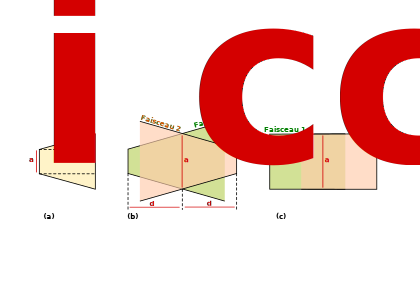
\includegraphics[width=\linewidth]{5-opti_theorique/divergence_luminosite.png}
	\caption{Illustrations de la collision de deux faisceaux avec une divergence, avec (a) la définition des quantités permettant de paramétriser le faisceau en forme de cône tronqué, (b) la collision de deux cônes tronqués, et (c) la collision de deux pavés équivalents sans divergence et d'arête $a_c$.}
	\label{fig:52-luminosite_divergence}
\end{figure}

Compte tenu de la forme des faisceaux, illustré en figure \ref{fig:52-luminosite_divergence}a, la taille de la source au point de collision peut donc être calculée comme étant :
\begin{equation}
    a_c=a_i+2d \tan \theta ~ \rm .
\end{equation}

En utilisant la formulation de la luminosité donnée par l'équation (\ref{eq:52-luminosite_contre_propagatif}), la luminosité de deux faisceaux divergeant d'un demi-angle $\theta$ collisionnant avec un angle $\psi_{12}=180^\circ$ à une distance $2d$ peut donc être estimée comme étant :
\begin{equation}
    \mathcal{L}_{12}^{sc} \sim \dfrac{N_1 N_2}{(a_i+2d\tan\theta)^2} ~ \rm .
    \label{eq:52-luminosite_divergence}
\end{equation}

La luminosité initiale est donc divisée d'un facteur $>10$ par rapport à une source identique avec une divergence nulle dès lors que $(a_i+2d\tan\theta)^2>10 ~ a_i^2$, ou encore $d > (\sqrt{10}-1) a_i/2\tan \theta \sim  1.1 ~ a_i/\tan \theta$. Pour une source de demi-angle de divergence 20 degrés et de taille 100 µm, pouvant représenter une source Bremsstrahlung \parencite{henderson_2014, ben-ismail_2011}, la distance de collision à partir de laquelle le nombre de paires est divisé par 10 est alors de l'ordre de l'ordre de $2d=600$ µm. Au contraire, pour une source de demi-angle de divergence 5 degrés et de taille 3 µm, pouvant représenter par exemple des sources de photons produites par un laser multi-PW se propageant dans un canal quasi-critique via le processus Compton inverse multi-photon \parencite{wang_2020}, la distance de collision à partir de laquelle le nombre de paires est divisé par 10 est de l'ordre de $2d=80$ µm. 

Ainsi, compte tenu de ces estimations, les sources produites par \textbf{Bremsstrahlung} seront a priori \textbf{les plus robustes à des variations de conditions expérimentales}, car celles-ci ont une \textbf{large extension spatio-temporelle} comparé aux autres types de sources (voir chapitre \ref{chap:2-laser}). Ce type de source semble alors le plus adapté à une \textbf{stratégie à haut taux de répétition}, car de petites variations de conditions expérimentales pourront apparaître entre différents tirs laser sans changer significativement le nombre de paires produites par tir. Néanmoins, et comme nous l'avons déjà évoqué, ces calculs font référence à la \textbf{variation} de la luminosité, et pas à la valeur absolue de luminosité en tant que telle, qui est plus importante pour des sources de faible extension spatio-temporelle, telles que e.g. les sources Compton-inverse multi-photon proposées par \cite{wang_2020}.

Dans cette section, nous avons vu que plusieurs stratégies peuvent être mises en place pour maximiser la luminosité, et donc le nombre de paires. Pour deux faisceaux donnés, et sans considérations de section efficace, le \textbf{nombre total de paires} est \textbf{maximisé} pour un \textbf{angle de collision de 180 degrés} et pour des sources collisionnant avec la \textbf{distance de collision la plus faible possible}. Les propriétés des faisceaux sont aussi d'une importance capitale, et ceux-ci devront exhiber au mieux un \textbf{nombre élevé de photons}, une \textbf{durée et une taille transverse faibles}, et une \textbf{divergence faible}.
Néanmoins, il est important de noter que la \textbf{luminosité} permet de caractériser la \textbf{collision de deux faisceaux}, et pas les propriétés d'un faisceau seul. Pour la collision de deux faisceaux de photons donnés, son calcul nécessite alors de fixer à la fois une distance et un angle de collision entre les sources.
Afin de pouvoir \textbf{comparer des sources de photons} entre elles \textbf{indépendamment des paramètres de la collision des faisceaux}, nous utiliserons dans le chapitre \ref{chap:6-opti_numerique} une quantité nommée \textbf{brillance crête à 1 MeV} (ou par abus de langage simplement brillance à 1 MeV), qui est exprimée en nombre de particules $\rm/s/mm^2/mrad^2/0.1\%BW$, où le terme $0.1\% \rm BW$ signifie $0.1  \%$ de largeur de bande en énergie (i.e. en considérant seulement les particules d'énergie comprise entre 0.995 MeV et 1.005 MeV). En effet, \textbf{la brillance} est \textbf{maximisée} pour un nombre important de photons d'énergie autour de 1 MeV, avec une extension spatio-temporelle du faisceau la plus faible possible et la divergence la plus faible possible, soit \textbf{pour des caractéristiques de faisceaux similaires à celles qui produisent une luminosité importante}. Ces deux quantités ne sont \textbf{néanmoins pas équivalentes}, comme cela peut être remarqué en tableau \ref{tab:52-luminosite_brillance} résumant la dépendance de la luminosité et de la brillance à diverses propriétés des faisceaux de photons.

\begin{table}
    \centering
    \begin{tabular}{ | l | l | l || l |}
    \hline
    & Luminosité eq. (\ref{eq:52-luminosite_pinceaux})  & Luminosité eq. (\ref{eq:52-luminosite_divergence})     & Brillance à 1 MeV                \\
    \hline
    Nombre de photons           & Oui           & Oui           & Oui           \\
    Rayon faisceaux             & Oui           & Oui           & Oui           \\
    Durée faisceaux             & Oui           & Non           & Oui           \\
    Divergence faisceaux        & Non           & Oui           & Oui           \\
    Énergies des photons        & Non           & Non           & Oui           \\
    Angle de collision          & Oui           & Non           & Non           \\
    Distance de collision       & Non           & Oui           & Non           \\
    \hline
	\end{tabular}
    \caption{Dépendance de la luminosité et de la brillance à diverses caractéristiques des faisceaux de photons.}
	\label{tab:52-luminosite_brillance}
\end{table}

Nous rappelons de plus que les formulations de la luminosité qui ont été développées ici permettent de donner des estimations rapides d'ordre de grandeurs mais ne doivent pas être vues comme des calculs quantitatifs, compte tenu des nombreuses hypothèses nécessaires et du cadre d'application très restreint de celles-ci. 

\section{Effets de la distribution en énergie des photons sur le nombre de paires}

En première partie de ce chapitre, nous avons vu que le nombre de paires produites par la collision de deux faisceaux de photons avec une distribution en énergie large et sans divergence peut s’écrire comme le produit d'une luminosité géométrique et d'une section efficace intégrée, définie dans l'équation (\ref{eq:51-sigma_int_definition}) comme :
\begin{equation}
    \sigma_{\gamma\gamma}^{int} = \iint_{0}^{+\infty} f_1 ~ f_2 ~ \sigma_{\gamma\gamma} ~ dE_1 ~ dE_2 ~ \rm ,
\end{equation}

avec $\sigma_{\gamma\gamma}$ la section efficace BWL, $E_i$ l'énergie du faisceau de photon $i$, et $f_i$ sa fonction de distribution en énergie (FDE), avec $i=\{1,2\}$.

Dans cette section nous verrons que, sous certaines conditions, $\sigma_{\gamma\gamma}^{int}$ peut être exprimée en fonction d'une seule variable, représentant le carré d'une énergie caractéristique de la collision. Certains cas particuliers seront alors étudiés plus en détail, et permettront d'apporter un éclairage intéressant sur l'optimisation de la distribution en énergie des sources de photons pour les expériences de création de paires BWL.

Sous certaines conditions, ce formalisme pourrait être réadapté pour l'étude d'autres processus de production de photons $\gamma$, de situations astrophysiques voire d'autres processus de collision de particules. 

\subsection{Principe}

Dans le cas général, le calcul de la section efficace intégrée définie par l'équation (\ref{eq:51-sigma_int_definition}) ne présente pas de solution directe, et la valeur de cette intégrale dépend principalement de la forme des FDE $f_1$ et $f_2$ considérées. Pour des raisons de simplicité, nous nous limiterons ici aux FDE pouvant s'exprimer en fonction d'un seul paramètre $K_i$ (ce paramètre étant ici appelé \textit{énergie caractéristique} du faisceau $i$) et que l'on peut exprimer sous la forme :
\begin{equation}
    f_i(E_i, K_i) = \dfrac{g_i(E_i/K_i)}{K_i} ~ \rm ,
    \label{eq:53-g_definition}
\end{equation}

avec $g_i$ une fonction à une seule variable (des exemples sont donnés dans le tableau \ref{tab:53-g_definitions}). Dans ce cadre, les conditions de normalisation pour $f_i$ et $g_i$ s'écrivent :
\begin{equation}
    \int_0^{+\infty} f_i (E_i, K_i) ~ dE_i = \int_0^{+\infty} g_i (E_i/K_i) ~ d(E_i/K_i) = 1 ~ .
    \label{eq:53-g_normalisation}
\end{equation}

L'équation (\ref{eq:51-sigma_int_definition}) peut alors être exprimée avec ses dépendances appropriées :
\begin{equation}
\sigma_{\gamma\gamma}^{int}(K_1, K_2, \psi_{12}) = \iint_0^{+\infty} \dfrac{g_1(E_1/K_1)}{K_1} \dfrac{g_2(E_2/K_2)}{K_2} ~ \sigma_{\gamma\gamma}(E_1, E_2, \psi_{12}) dE_1 dE_2 ~ .
\label{eq:53-sigma_int_dependances}
\end{equation}

Pour l'intégrale double d'une fonction $F(u,v)$ sur un domaine $V$, il est possible (sous certaines conditions) de remplacer les variables d'intégration $(u,v)=\varphi(x,y)$ par les variables $(x,y)$ via le théorème de changement de variables \parencite{appel_2008} :
\begin{equation}
    \iint_V F(u,v) ~ du ~ dv = \iint_U F \circ \varphi(x,y) ~ |J_\varphi(x,y)| ~ dx ~ dy ~ \rm ,
    \label{eq:53-theoreme_changement_variable}
\end{equation}

où $U$ est le domaine d'intégration sur $(x,y)$, où l'opération $\circ$ est l'opération de composition des fonctions, et où $J_\varphi$ est le déterminant Jacobien de la transformation défini par :
\begin{equation}
J_\varphi = 
    \begin{vmatrix}
    \dfrac{\partial u}{\partial x}    & \dfrac{\partial u}{\partial y} \\
    \dfrac{\partial v}{\partial x}    & \dfrac{\partial v}{\partial y} \\
    \end{vmatrix} ~ \rm .
\end{equation}

En se rappelant que $s=2 E_1 E_2 (1-\cos{\psi_{12}})$, et en définissant de nouvelles variables $\eta=2 K_1 E_2 (1-\cos{\psi_{12}})$ et $\zeta=2 K_1 K_2 (1-\cos{\psi_{12}})$, on peut alors effectuer un changement de variable remplaçant les variables $E_1$ et $E_2$ par $s$ et $\eta$, où $(E_1,E_2)$ correspond à $(u,v)$ dans la définition précédente et où $(s,\eta)$ correspondent à $(x,y)$. Comme $E_1= K_1 ~ s/\eta$ et que $E_2=K_2 ~ \eta/\zeta$, le déterminant Jacobien $J$ de ce changement de variable est :
\begin{equation}
J_\varphi = 
    \begin{vmatrix}
    \dfrac{\partial E_1}{\partial s}    & \dfrac{\partial E_1}{\partial \eta} \\
    \dfrac{\partial E_2}{\partial s}    & \dfrac{\partial E_2}{\partial \eta} \\
    \end{vmatrix}
    =
    \begin{vmatrix}
    \dfrac{K_1}{\eta}       			& -K_1\dfrac{s}{\eta^2} \\
    0               					& ~ \dfrac{K_2}{\zeta} \\
    \end{vmatrix}
    =\dfrac{K_1}{\eta} \dfrac{K_2}{\zeta} ~ \rm .
\end{equation}

Par application du théorème du changement de variables (\ref{eq:53-theoreme_changement_variable}), et en utilisant la définition de $\sigma_{\gamma\gamma}^{int}$ de l'équation (\ref{eq:53-sigma_int_dependances}), on obtient donc :
\begin{equation}
    \sigma_{\gamma\gamma}^{int}(\zeta) = \dfrac{1}{\zeta} \int_0^{+\infty} g_2(\eta/\zeta) \left[\dfrac{1}{\eta} \int_0^{+\infty} g_1(s/\eta) \sigma_{\gamma\gamma}(s) ds \right] d\eta ~ .
    \label{eq:53-sigma_int_s_eta}
\end{equation}

Ainsi, pour des fonctions de la forme indiquée par l'équation (\ref{eq:53-g_definition}), la section efficace intégrée $\sigma_{\gamma\gamma}^{int}$ peut être exprimée \textbf{en fonction d'un seul paramètre} $\zeta=2 K_1 K_2 (1-\cos{\psi_{12}})$. Ce paramètre est défini par analogie avec la variable de Mandelstam $s=2E_1 E_2 (1-\cos\psi_{12})=E_{CM}^2$ et peut donc être vu comme une énergie caractéristique de la collision au carré $\zeta = K_{CM}^2$, avec $K_{CM}$ une énergie caractéristique de la collision. 

Nous avons vu au début de ce chapitre que le nombre de paires produites dans la collision de deux faisceaux de photons est directement proportionnel à la section efficace intégrée $\sigma_{\gamma\gamma}^{int}$, et il pourra donc être intéressant d'optimiser les caractéristiques énergétiques des sources de photons de façon à la maximiser. La valeur du paramètre $\zeta$ maximisant $\sigma_{\gamma\gamma}^{int}$ sera notée $\zeta'$.

Dans la suite, nous calculerons numériquement l'intégrale donnée par l'équation (\ref{eq:53-sigma_int_s_eta}) pour quelques fonctions $g_1$ et $g_2$ d'intérêt pour la collision de faisceaux de photons en laboratoire. Les valeurs numériques obtenues seront aussi approximées par une fonction d'ajustement, afin de pouvoir être réutilisées facilement par la suite. 

\subsection{Application à la collision de faisceaux de photons en laboratoire}

Nous allons maintenant appliquer ces résultats à des situations de collision de faisceaux de photons en laboratoire, en particulier dans les propositions de schéma expérimentaux faisant intervenir des sources de photons directionnelles ; mieux adaptées au formalisme de la luminosité. Pour pouvoir étudier ces configurations à l'aide de l'équation (\ref{eq:53-sigma_int_s_eta}), nous aurons tout d'abord besoin de déterminer des formes de distribution en énergie de photons $f_i$ satisfaisant les conditions définies à la fois par l'équation (\ref{eq:53-g_definition}) et par l'équation (\ref{eq:53-g_normalisation}). Nous discuterons particulièrement des propositions faisant intervenir deux sources Bremsstrahlung produites par laser \parencite{ribeyre_2016}, deux sources Compton inverse linéaire produites par le couplage d'un collisionneur à électrons avec deux lasers \parencite{drebot_2017a}, ou deux sources produites par le processus Compton inverse multi-photon dans l'interaction d'un laser de classe PW se propageant dans un micro-canal \parencite{wang_2020} :
\begin{enumerate}[label=\roman*. ]
    \item Pour modéliser la distribution en énergie de photons produits par le processus \textbf{Bremsstrahlung}, nous considérons une fonction de forme \textbf{exponentielle décroissante}, telle que définie dans le tableau \ref{tab:53-g_definitions}. Ce type de fonction, qui satisfait à la fois les conditions de l'équation (\ref{eq:53-g_definition}) et de l'équation (\ref{eq:53-g_normalisation}), est en effet usuellement utilisé dans la littérature \parencite{norreys_1999, zulick_2013, henderson_2014} pour décrire les mesures de distributions en énergie de ce type de sources, où la pente de l'exponentielle est parfois appelée \textit{température effective}, mais sera ici appelé \textit{énergie caractéristique} et sera notée $K$. Un exemple de ce type d'ajustement de courbe est affiché en figure \ref{fig:53-exemples_f}a, où deux exponentielles ont été utilisées pour décrire respectivement la partie haute et basse énergie des données mesurées \parencite{zulick_2013}. D'autres formulations analytiques existent néanmoins pour décrire les sources de photons produites par Bremsstrahlung dans des cibles fines \parencite{shkolnikov_1997} ou épaisses \parencite{matthews_1973, findlay_1989, tsai_1974}, mais celles-ci ne satisfont en pas en général les deux conditions données par les équations (\ref{eq:53-g_definition}) et (\ref{eq:53-g_normalisation}).
    
    \item Les sources de photons obtenues par propagation d'un \textbf{laser multi-PW dans un micro-canal} sont quant à elles modélisées par une fonction de la forme d'une \textbf{loi de puissance multipliée par une exponentielle décroissante}, dont la formulation précise est indiquée dans le tableau \ref{tab:53-g_definitions}. Ce type de fonction satisfait les conditions des équations (\ref{eq:53-g_definition}) et (\ref{eq:53-g_normalisation}), et permet de raisonnablement reproduire les données obtenues à l'aide de simulations 3D décrites dans la référence \cite{wang_2020}, en particulier la simulation avec un laser de puissance 2 PW. Ces données, obtenues et reproduites avec la courtoisie de T. Wang, sont affichées en figure \ref{fig:53-exemples_f}b. Nous pouvons remarquer que l'utilisation de ce type de fonction permet de reproduire les données de 10 keV à 10 MeV (voir "Fit LMC" en figure \ref{fig:53-exemples_f}b) si on considère une seule fonction du type de celle définie dans le tableau \ref{tab:53-g_definitions}, ou de 10 keV à 100 MeV si on considère la somme de deux fonctions de ce type (voir "Fit 2 LMC" en figure \ref{fig:53-exemples_f}b). L'adaptation de notre formalisme à l'utilisation d'une somme de fonctions est discutée en annexe \ref{an:5-somme_2_fonctions}. Ce type de sources de photons est parfois appelé "sources de type synchrotron", ou \textit{synchrotron-like} dans la littérature, et la distribution en énergie de photons émis par rayonnement synchrotron d'un électron en mouvement circulaire instantané (voir \parencite{jackson_2009}) peut satisfaire à la fois les conditions des équations (\ref{eq:53-g_definition}) et (\ref{eq:53-g_normalisation}). Néanmoins, cette fonction de distribution en énergie reproduit moins bien ces données de simulation que la fonction que nous proposons en tableau \ref{tab:53-g_definitions}.
    
    \item Enfin, les sources produites par le processus \textbf{Compton inverse linéaire} sont modélisées par une \textbf{distribution en énergie constante jusqu'à une énergie maximale}, appelée énergie caractéristique et notée $K$. Ce type de fonction de distribution, décrite dans le tableau \ref{tab:53-g_definitions}, permet d'approximer très grossièrement les données obtenues à l'aide de simulations numériques par \cite{drebot_2017a}, et affichées en figure \ref{fig:53-exemples_f}c. Des formulations analytiques plus précises permettent néanmoins de modéliser les sources de photons produites par diffusion de photons laser par un faisceau d'électron \parencite{fargion_1997}, mais celles-ci ne satisfont pas les conditions données par les équations (\ref{eq:53-g_definition}) et (\ref{eq:53-g_normalisation}).
\end{enumerate}

\begin{figure}[hb]
	\centering
	\includegraphics[width=\linewidth]{5-opti_theorique/gamma_energy_distribution.png}
	\caption{Illustration des fonctions d'ajustement choisies pour modéliser (a) des sources de photons produites par Bremsstrahlung, (b) des sources de photons produites par propagation d'un laser multi-PW dans un micro-canal, et (c) des sources de photons produites par le processus Compton inverse linéaire d'un faisceau d'électrons sur un laser. La formulation mathématique des fonctions correspondantes est donné au tableau \ref{tab:53-g_definitions}, et celles-ci sont affichées en figure \ref{fig:53-sigma_int_resultats}a. Les figures (a) et (c) proviennent respectivement de \parencite{zulick_2013} et de \parencite{drebot_2017a}, et la figure (b) a été produite grâce aux données gracieusement partagées par T. Wang, et décrites dans \parencite{wang_2020}.} 
	\label{fig:53-exemples_f}
\end{figure}

La forme de la fonction $g_i(E_i/K_i)$ est aussi tracé en figure \ref{fig:53-sigma_int_resultats}a pour ces trois types de distributions en énergie.

\begin{table}[t]
    \centering
    \begin{tabular}{ | l | l | l | l |}
    \hline
                & Type de FDE (\textit{Abréviation})       & Forme mathématique de $g_i(E_i/K_i)$ \\
    \hline
    \textit{I}   & Bremsstrahlung (\textit{Brem})           & $\exp(-E_i/K_i)$ \\
    \textit{II}  & Laser dans un micro-canal (\textit{LMC}) & $\dfrac{1}{\Gamma(0.05)} \times \left(\dfrac{E_i}{K_i}\right)^{-0.95} \times \exp\left(-\dfrac{E_i}{K_i}\right)$ \\
    \textit{III} & Compton inverse linéaire (\textit{CIL})  & $\left\{\begin{array}{@{}ll@{}} 1 & \text{si}\ E_i/K_i < 1 \\0 & \text{sinon}\end{array}\right.$ \\
    \hline
	\end{tabular}
    \caption{Définition des fonctions de distributions en énergies (FDE) utilisés pour modéliser les différentes sources de photons. $\Gamma$ est la fonction gamma.}
	\label{tab:53-g_definitions}
\end{table}

Pour ces définitions, nous pouvons alors modéliser l'interaction de deux sources de type Bremsstrahlung (noté \textit{Brem}), deux sources produites par un laser se propageant dans un micro-canal (noté \textit{LMC}), ou deux sources produites par Compton inverse linéaire (noté \textit{CIL}), en insérant ces définitions dans l'expression de la section efficace intégrée (\ref{eq:53-sigma_int_s_eta}). Cette intégration a été effectuée sur 300 points espacés logarithmiquement entre $10^{-2}$ et $10^{12} ~ \rm MeV^2$, et ces résultats sont affichés en fonction de $\sqrt{\zeta}=\sqrt{2 K_1 K_2 (1-\cos{\psi_{12}})}$ en $\rm MeV$ en figure \ref{fig:53-sigma_int_resultats}b.

\begin{figure}[hbtp]
	\centering
	\includegraphics[width=\linewidth]{5-opti_theorique/resultats.png}
	\caption{Les fonctions de distributions en énergie $g_i$ définies dans le tableau \ref{tab:53-g_definitions} sont affichées en (a), et les sections efficaces intégrées correspondantes, calculées à partir de l'équation (\ref{eq:53-sigma_int_s_eta}), sont affichées en (b) en fonction de $\sqrt{\zeta}$. Sur cette figure, les ronds bleus correspondent aux données obtenues numériquement en considérant deux FDE de type \textit{Brem}, les carrés mauves aux données obtenues en considérant deux FDE de type \textit{CIL}, et les losanges rouges aux données obtenues en considérant deux FDE de type \textit{LMC}. Les traits pleins correspondent à l'ajustement des données numériques avec l'équation (\ref{eq:53-h_definition}), et les tirets noirs à la section efficace pour la collision de deux faisceaux mono-énergétiques, soit la section efficace BWL donnée par l'équation (\ref{eq:51-sigma_BWL}) avec $\zeta=s$. Le médaillon est un zoom sur l'intervalle $\sqrt{\zeta}\in[10^{-1},10^2]$ avec une échelle des ordonnées linéaire.}
	\label{fig:53-sigma_int_resultats}
\end{figure}

Pour pouvoir interpréter ces résultats et estimer l'effet de la distribution en énergie des photons sur la création de paires électron-positron, il pourrait être intéressant de disposer d'un \textbf{cas de référence} considérant deux faisceaux de photons de \textbf{distributions en énergies mono-énergétiques}. Ceux-ci peuvent être décrits par une distribution de Dirac $f_i(E_i, K_i) = \delta(E_i/K_i-1)$ pour chaque faisceau, et l'intégrande de l'équation (\ref{eq:51-sigma_int_definition}) est dans ce cas non nulle uniquement pour $E_i=K_i$. Pour la collision de deux faisceaux mono-énergétiques, la section efficace intégrée  (\ref{eq:51-sigma_int_definition}) se réduit donc à la \textbf{section efficace BWL} (\ref{eq:51-sigma_BWL}), et notre variable $\zeta$ est équivalente à la variable de Mandelstam $s$. Nous pouvons alors tracer la section efficace BWL donnée par l'équation (\ref{eq:51-sigma_BWL}) sur la même figure que les résultats obtenus à partir de l'équation (\ref{eq:53-sigma_int_s_eta}), et ainsi comparer nos sections efficaces intégrées à ce cas de référence considérant deux faisceaux mono-énergétiques.


Les résultats affichés en figure \ref{fig:53-sigma_int_resultats}b tendent à montrer que, pour des faisceaux de photons de \textbf{distribution en énergies larges} (par exemple pour le cas \textit{Brem}-\textit{Brem}), la section efficace intégrée est \textbf{moins piquée} que la section efficace BWL, et son \textbf{amplitude maximale plus faible}. Une variation d'angle ou d'énergie caractéristique a donc une influence plus limitée sur le nombre total de paires produites que pour deux faisceaux mono-énergétiques. La réduction de l'amplitude maximale indique aussi que, toutes choses égales par ailleurs, le nombre de paires produites dans la collision de deux faisceaux de photons avec des distributions en énergie larges est aussi plus faible.

Pour expliquer qualitativement ces comportements, considérons tout d'abord la collision de deux faisceaux mono-énergétiques sans divergence. Dans ce cas, l'\textbf{énergie} et l'\textbf{angle de collision} des photons incidents est \textbf{identique pour chaque collision binaire} (i.e. pour chaque collision entre seulement deux photons de faisceaux différents). La valeur de la variable de Mandelstam $s=2 E_1 E_2 (1-\cos\psi_{12})$ est elle aussi identique pour toutes ces collisions binaires, et la section efficace de création de paires dans la collision de ces deux photons (section efficace BWL) est donc la même pour toutes les collisions binaires ayant lieu lors de l'interaction des deux faisceaux. En choisissant convenablement les valeurs d'énergies et d'angle, il est donc possible de maximiser la section efficace BWL pour chaque collision binaire. Au contraire, dans la collision de faisceaux de photons avec des distributions en énergies larges (e.g. de forme \textit{Brem}, \textit{LMC} ou \textit{CIL}), la valeur de $s$ \textbf{peut varier} entre chaque collision binaire, et la section efficace de création de paires par collision de deux photons (section efficace BWL) \textbf{ne peut plus être maximisée dans chacune de ces collisions binaires}. La section efficace intégrée, modélisant la probabilité \textbf{totale} de création de paires dans la collision des deux \textbf{faisceaux}, a donc une amplitude plus faible par rapport à la section efficace pour deux faisceaux de photons mono-énergétiques, qui est égale à la section efficace BWL.

La création de paires par collision de \textbf{deux} photons présente aussi un seuil de production pour $s = 2 E_1 E_2 (1-\cos{\psi_{12}})\ge (2 m_e c^2)^2$, et seules les collisions binaires satisfaisant cette inégalité peuvent contribuer la production de paires totale (voir chapitre \ref{chap:1-particules}). Ainsi, les photons de plus \textbf{basse énergie} peuvent contribuer à la production de paires \textbf{uniquement} si ils collisionnent avec un photon de \textbf{haute énergie}, et les collisions \textbf{entre photons de basse énergies} ne seront \textbf{pas utiles} pour notre application.

Pour des distributions en énergies larges, la densité de probabilité pour que les énergies des photons dans une collision binaire donnée soit comprise entre $(E_1,E_2)$ et $(E_1+dE_1, E_2+dE_2)$ est définie par le produit $f_1 \times f_2$. Pour deux distributions en énergie de type \textbf{\textit{CIL}} (constantes jusqu'à une énergie maximale), cette densité de probabilité est \textbf{non nulle seulement} pour des couples d'énergie $(E_1, E_2)$ situés \textbf{dans une zone délimitée par les deux bornes supérieures en énergie} $K_1$ et $K_2$. Cette configuration est illustrée en figure \ref{fig:53-exemples_FDE}c pour $K_1=K_2=3 ~ \rm MeV$, où les lignes obliques indiquent le seuil de production de paires, la section efficace maximale, et la valeur pour laquelle la section efficace à une valeur inférieure à $1/10$ de son maximum, pour un angle $\psi_{12}=180^\circ$. Cette configuration correspond alors à une valeur de $\zeta$ de $2 \times 3 \times 3 \times 2 = 36 ~ \rm MeV^2$. Comme nous pouvons le remarquer sur cette figure, \textbf{seule une proportion des collisions binaires} d'énergies $(E_1,E_2)$ sont \textbf{situées au delà du seuil de création de paires} et \textbf{sont donc réellement utiles} pour la production de paires électron-positron. 
En prenant l'exemple de la figure \ref{fig:53-exemples_FDE}c pour référence, et pour un angle de collision $\psi_{12}$ fixé, la \textbf{diminution} de la valeur des \textbf{énergies caractéristiques} $K_1$ et $K_2$ (et donc la diminution de la valeur de $\zeta$) aura tendance à \textbf{diminuer la proportion de couples d'énergies au dessus du seuil de création de paires}, car les bornes délimitant la \textbf{zone de probabilité non nulle} se déplacent vers des \textbf{valeurs d'énergies plus faibles}. Pour une valeur de $\zeta=2K_1 K_2 (1- \cos{\psi_{12}})< (2 m_e c^2)^2$, \textbf{aucun couple d'énergie} $(E_1,E_2)$ de probabilité non nulle n'est \textbf{au dessus du seuil de création de paires}, et le \textbf{nombre de paires} produites doit être \textbf{strictement nul}. Ce \textbf{comportement de seuil} est bien représenté dans les résultats de la figure \ref{fig:53-sigma_int_resultats}b, où la section efficace intégrée peut être comprise comme le produit de la fonction à deux dimensions représenté sur la figure \ref{fig:53-exemples_FDE}c, multipliée par la section efficace BWL, et intégré sur toutes les énergies (voir équation (\ref{eq:53-sigma_int_dependances})). 
Au contraire, si les valeurs des \textbf{énergies caractéristiques} $K_1$ et $K_2$ \textbf{augmentent} (et donc que $\zeta$ augmente), une \textbf{plus grande proportion de couples d'énergies} $(E_1,E_2)$ se retrouvent \textbf{au dessus du seuil de création de paires} $s=2 E_1 E_2 (1- \cos{\psi_{12}}) > (2 m_e c^2)^2$, et on pourrait s'attendre à une augmentation de la section efficace intégrée. Néanmoins, la \textbf{collision de photons de trop hautes énergies} n'est \textbf{pas optimale} pour la création de paires, car la\textbf{ probabilité de création de paires} (i.e. la section efficace BWL) \textbf{diminue pour des valeurs de $s$ trop élevées} (lorsque $\sqrt{s}>1.43 ~ \rm MeV$). Pour des valeurs de $K_1$ et $K_2$ trop importantes (i.e. pour des valeurs de $\zeta$ trop élevées), une \textbf{proportion importante des collisions binaires entre photons} pourrait être \textbf{très peu efficace pour la création de paires}, et la \textbf{probabilité de création de paires totale} (modélisée par la section efficace intégrée) aurait dans ce cas tendance à \textbf{diminuer} (on rappelle que la distribution en énergie est normalisée, et qu'une augmentation de la proportion de collisions binaires entre photons de hautes énergies induit donc en contrepartie une diminution de la densité de probabilité dans les zones de plus faibles énergies, où la probabilité de création de paires est plus importante). 
Ainsi, au delà du seuil donné par la condition $\sqrt{\zeta}>2 m_e c^2$, l'augmentation de $\zeta$ a tout d'abord un effet bénéfique sur la création de paires totale car elle permet d'augmenter la proportion de collisions de photons ayant une énergie suffisante pour produire des paires. Néanmoins, pour des valeurs de $\zeta$ trop importantes, une grande proportion des collisions binaires ont lieu entre photons de hautes énergies, qui produisent peu de paires. La section efficace intégrée est donc \textbf{croissante} pour des faibles valeurs de $\zeta$ au delà du seuil, puis atteint donc une \textbf{valeur maximale}, et \textbf{décroît} pour des valeurs de $\zeta$ importantes, tel que ceci est observé sur la figure \ref{fig:53-sigma_int_resultats}.

Pour des collisions de faisceaux de photons avec des distributions en énergies larges et \textbf{décroissantes monotones}, telles que les FDE notées \textit{Brem} et \textit{LMC} les fonctions de distributions en énergie n'exhibent \textbf{pas de borne supérieure en énergie}. La probabilité d'obtenir un couple d'énergie situé entre $(E_1,E_2)$ et $(E_1+dE_1, E_2+dE_2)$ par un tirage aléatoire est représenté respectivement en figures \ref{fig:53-exemples_FDE}a et \ref{fig:53-exemples_FDE}b pour ces deux types de fonctions, où on a fixé $K_1=K_2=3 ~ \rm MeV$. Pour un angle de collision fixé, une diminution des énergies caractéristiques $K_1$ et $K_2$ (représentant maintenant les pentes, ou \textit{températures effectives} de ces distributions en énergies) fera donc diminuer la proportion de couples de photons au delà du seuil de création de paires, mais la probabilité d'obtenir un couple d'énergies au dessus du seuil de création de paires ne sera néanmoins jamais rigoureusement nulle. Ainsi, on n'observe \textbf{pas de comportement de seuil de création de paires} dans la section efficace intégrée représentant la collision de ce type de faisceaux, tel qu'on peut le remarquer en figure \ref{fig:53-sigma_int_resultats}b. De la même manière que précédemment, une augmentation trop importante de $K_1$ et $K_2$ (et donc de $\zeta$) aura tendance à favoriser les couples d'énergies de photons situés dans des zones ou la section efficace BWL est faible. La section efficace intégrée est alors croissante pour des faibles valeurs de $\zeta$, puis atteint un maximum avant de décroître pour des valeurs de $\zeta$ plus importantes (cet effet n'est pas clair sur la figure \ref{fig:53-sigma_int_resultats}b pour le cas \textit{LMC-LMC}, mais celui-ci atteint bien son maximum entre $\sqrt{\zeta} \sim 10^5 ~ \rm MeV$ et $\sqrt{\zeta} \sim 10^6 ~ \rm MeV$).

\begin{figure}[hbtp]
	\centering
	\includegraphics[width=\linewidth]{5-opti_theorique/exemples_FDE.png}
	\caption{Probabilité d'obtenir une valeur d'énergie entre $(E_1,E_2)$ et $(E_1+dE_1, E_2+dE_2)$ pour (a) deux FDE de type \textit{Brem}, (b) deux FDE de type \textit{LMC} et (c) deux FDE de type \textit{CIL}, avec $K_1=K_2=3 ~ \rm MeV$ et $\psi_{12}=180$ degrés.}
	\label{fig:53-exemples_FDE}
\end{figure}

Ainsi, les trois cas considérés présentent une valeur de $\zeta=2 K_1 K_2 (1-\cos\psi_{12})$ notée $\zeta'$ qui maximise la section efficace intégrée (\ref{eq:53-sigma_int_s_eta}), et qui est indiquée en tableau \ref{tab:53-h_fit}. Le nombre de paires produites étant directement proportionnel à la section efficace intégrée (cf équation (\ref{eq:51-N+_definition})), il est alors possible d'\textbf{optimiser les énergies caractéristiques} des distributions en énergies des photons en satisfaisant la condition :
\begin{equation}
2 K_1 K_2 (1-\cos\psi_{12})=\zeta' ~ \rm .
\end{equation}


En fixant l'\textbf{angle de collision à $\psi_{12}=180$ degrés} et en supposant la collision de deux sources de photons \textbf{identiques} ($K_1=K_2$), il est donc possible d'estimer les \textbf{énergies caractéristiques} permettant de \textbf{maximiser la production de paires} :

\begin{enumerate}[label={\Roman*. }]
    \item Pour deux sources produites par Bremsstrahlung, modélisées ici par des exponentielles (voir table \ref{tab:53-g_definitions}), l'optimum de $\zeta$ se situe autour de $\zeta' \sim 8.00 ~ \rm MeV^2$. Ainsi, pour deux sources de photons identiques contra-propagatives, les énergies caractéristique $K_i$ (correspondant à la pente de l'exponentielle) permettant de maximiser la production de paires électron-positron sont de l'ordre de $1.4 ~ \rm MeV$. Dans le cadre de l'interaction laser-plasma à haute intensité, ce type d'énergies caractéristiques a \textbf{déjà été obtenu expérimentalement dès la fin des années 1990} \parencite{norreys_1999}. La \textbf{valeur maximale de section efficace intégrée} correspondante est \textbf{de l'ordre de $r_e^2$}, soit seulement $2$ fois moins importante que la valeur maximale pouvant être obtenue en considérant la collision de deux faisceaux mono-énergétiques.
    
    \item L'optimum de section efficace intégrée pour la collision de deux sources de type \textit{LMC} est quant à lui situé pour des énergies caractéristiques $K_i$ de l'ordre de $5 \times 10^{4} ~ \rm MeV$, en considérant des faisceaux identiques contra-propagatifs. Ces valeurs d'énergies caractéristiques sont alors \textbf{très largement supérieures} aux valeurs obtenues par ajustement des données de \cite{wang_2020} (voir figure \ref{fig:53-exemples_f}), qui sont typiquement autour de quelques MeV à quelques dizaines de MeV. Néanmoins, nous pouvons le remarquer en figure \ref{fig:53-sigma_int_resultats}b que pour des valeurs de $\zeta$ importantes, la section efficace intégrée est \textbf{quasiment constante}, et atteint environ $1/2$ fois sa valeur maximale autour de $\zeta \approx 43 ~ \rm MeV^2$. Les valeurs d'énergies caractéristiques correspondant $\zeta \sim 40 ~ \rm MeV^2$ sont bien plus raisonnables, autour de $3 ~ \rm MeV$, et sont typiquement de l'ordre de grandeur des valeurs obtenues via l'ajustement des données affiché en figure \ref{fig:53-exemples_f}b. La section efficace correspondant au \textbf{maximum de section efficace intégrée} est ici \textbf{de l'ordre de $0.1 ~ r_e^2$}, soit environ $20$ fois moins que le cas idéal de collision de faisceaux mono-énergétiques.
    
    \item En considérant la collision de sources produites par le processus Compton inverse linéaire, modélisées par des distributions en énergies constantes jusqu'à une borne maximale, l'optimum de section efficace intégrée est atteint pour $\zeta' \sim 15.3 ~ \rm MeV^2$, soit pour des valeurs d'énergies caractéristiques (i.e. de borne supérieure de la distribution en énergie dans ce cas) de l'ordre de $1.9 ~ \rm MeV$. Dans leur article, les auteur$\cdot$es \cite{drebot_2017a} considèrent la diffusion Compton inverse linéaire d'un laser de longueur d'onde $1 ~ \rm \mu m$ par des électrons d'énergie autour de $260 ~ \rm MeV$, pouvant donc produire des photons d'énergie jusqu'à $\sim 1.2 ~ \rm MeV$ (cette valeur est déterminée par la cinématique de la collision). Cette valeur d'énergie caractéristique semble alors très légèrement sous-optimale, et dans notre modélisation le nombre total de paires produites serait diminué raisonnablement d'un facteur $\sim 1.2$. Pour atteindre la valeur optimale d'énergie caractéristique donné par notre modèle, le faisceau d'électrons devrait avoir une énergie autour de $325 ~ \rm MeV$, en supposant un laser diffusé de même longueur d'onde. Ce type d'énergie a ici aussi \textbf{déjà été atteintes en laboratoire} \parencite{albert_2016}. La \textbf{section efficace intégrée} est ici \textbf{maximisée avec une valeur de l'ordre de $r_e^2$}, et correspond ici aussi à une réduction du nombre de paires d'un facteur $2$ comparé au cas idéal de la collision de faisceaux mono-énergétiques.
\end{enumerate}

Ainsi, à première vue les sources Bremsstrahlung et Compton inverse linéaire semblent particulièrement adaptées à la création de paires électron-positron par collision de photons, puisque la section efficace intégrée a une valeur maximale importante autour de $r_e^2$, et ce maximum peut être atteint en considérant des valeurs d'énergies caractéristiques réalistes. Les sources produites par propagation d'un laser multi-PW dans un micro-canal ont quant à elles une valeur de section efficace intégrée inférieure d'un ordre de grandeur, et la position du maximum correspond à des énergies caractéristiques hors d'atteinte expérimentalement. Néanmoins, cette section efficace intégrée présente une très faible variation pour des valeurs importantes de $\zeta$, et des valeurs d'énergies caractéristiques réalistes permettent d'atteindre des valeurs de section efficace intégrée étant une fraction significative de sa valeur maximale. De plus, ce type de source peut aussi présenter un grand nombre de photons avec une divergence angulaire et une extension spatiale modérée, ce qui peut conduire à un nombre de paires produites significatif malgré une section efficace intégrée moins importante.

En particulier, le cas avec un laser de 2 PW décrit dans \cite{wang_2020} présente un nombre de photons d'énergie $>10 ~ \rm keV$ de l'ordre de $2 \times 10^{12}$, avec une extension spatiale initiale qui peut être estimée comme étant de l'ordre de la tache focale du laser, soit autour de $2 ~ \rm \mu m$. En considérant un demi-angle de divergence de $5$ degrés, une distance de collision de $500 ~ \rm \mu m$ (chaque source est située à une distance $d=250 ~ \rm \mu m$ du plan de collision), et avec l'équation (\ref{eq:52-luminosite_divergence}), on obtient une luminosité simple collision de l'ordre de $2 \times 10^{29} ~ \rm cm^{-2}$. En supposant une section efficace de l'ordre de $0.1 ~ r_e^2$, le nombre de paires produites par tir est alors de l'ordre de $2\times 10^3$, soit du \textbf{même ordre de grandeur} que les estimations considérées dans la référence \parencite{wang_2020} pour un angle de collision de $90$ degrés.

En considérant un laser de la même gamme d'énergie, soit 80 J, interagissant avec un bloc solide de tantale ($Z=73$) d'épaisseur millimétrique, les auteur$\cdot$es \cite{palaniyappan_2019} ont mesuré les caractéristiques d'une source de photons produits par le processus Bremsstrahlung, et rapportent une énergie caractéristique (ou température effective) des photons de quelques $\rm MeV$, un demi-angle de divergence typique de l'ordre de $10$ degrés (ou $\sim 0.1 ~ \rm sr$), une taille typique de l'ordre de $80 ~ \rm \mu m$, avec un nombre de photons de l'ordre de $6 \times 10^{11}$ (de l'ordre de $3 \times 10^{12}$ par $\rm sr$, avec un demi-angle de divergence de $0.1 ~ \rm sr$). En considérant la collision de deux de ces sources à une distance de $500 ~ \rm \mu m$ (chaque source est située à une distance $d=250 ~ \rm \mu m$ du plan de collision), on peut alors estimer que la luminosité correspondante est de l'ordre de $1 \times 10^{27} ~ \rm cm^{-2}$. Pour une section efficace intégrée typique, de l'ordre de $r_e^2$, on peut alors estimer le nombre de paires produites par tir comme étant de l'ordre de $100$ paires par tir. Ainsi, les \textbf{sources Bremsstrahlung} exhibent un \textbf{nombre de paires inférieur} d'un ordre de grandeur au cas précédent d'un \textbf{laser dans un micro-canal}, en supposant un \textbf{laser d'énergie similaire}, et ce \textbf{malgré une section efficace intégrée dix fois supérieure} pour les sources Bremsstrahlung. Ces estimations tendent aussi à être très inférieures aux estimations obtenues via le modèle de \cite{ribeyre_2016}, qui ne prenaient pas en compte la taille initiale de la source ni les effets de distribution en énergie des photons, et qui donne dans ce cas un nombre de paires par tir de l'ordre de $10^5$, en supposant un faisceau de photons d'énergie totale $0.8 ~ \rm J$.

Enfin, en considérant les sources de photons obtenues via le processus Compton inverse linéaire par \cite{drebot_2017a}, avec une taille initiale typique de l'ordre de $10 ~ \rm \mu m$, un demi-angle de divergence typique de $5 ~ \rm mrad \sim 0.3$ degrés et un nombre de photons de l'ordre de $2 \times 10^9$ (ce nombre a été obtenu à partir de la référence \parencite{micieli_2016a} présentant des caractéristiques légèrement différentes), la luminosité simple collision à une distance de $8 ~ \rm mm$, est de l'ordre de $9 \times 10^{22} ~ \rm cm^{-2}$ et le nombre de paires est d'environ $10^{-2}$ par tir (en supposant une section efficace intégrée de $r_e^2$). Cette estimation est alors supérieure d'environ deux ordres de grandeur à celle obtenue à l'aide de \textbf{simulations numériques} dans la référence \parencite{drebot_2017a}, où la création de paires par collision de photons est modélisée de manière bien plus réaliste que notre modèle.

Compte tenu des nombreuses hypothèses simplificatrices effectuées pour ces calculs (à la fois pour la luminosité et pour la section efficace intégrée), il est néanmoins nécessaire de ne pas prendre ces nombres de paires pour des estimations trop quantitatives, mais plutôt comme des \textbf{outils utiles} pour déterminer dans quelle mesure une source de photons donnée pourrait être intéressante pour l'application de la création de paires par BWL. Ces estimations ne sauraient donc se substituer à des études plus poussées, prenant en compte une distribution en énergie plus réaliste et surtout la divergence des sources, particulièrement importante pour les sources Bremsstrahlung. Les valeurs obtenues par l'intermédiaire de ce modèle sont néanmoins cohérentes avec les données disponibles dans la littérature.

Les données obtenues par intégration numérique de l'équation (\ref{eq:53-sigma_int_s_eta}) peuvent aussi être ajustés avec une fonction de la forme de :
\begin{equation}
h(\zeta) = r_e^2 \times (a / \zeta^n) \times \exp\left(-b / \zeta^m \right) ~ \rm ,
\label{eq:53-h_definition}
\end{equation}

où $a$, $b$, $n$ et $m$ sont des réels positifs. Cette fonction est représentée en figure \ref{fig:53-sigma_int_resultats}b, avec les paramètres $a$, $b$, $n$ et $m$ indiqués dans le tableau \ref{tab:53-h_fit}. Nous pouvons noter que l'\textbf{ajustement des données} est \textbf{très raisonnable} dans les trois cas pour des valeurs de section efficace intégrée $\gtrsim 10^{-2} ~ r_e^2$. Cette fonction pourra donc être réutilisée pour mener des estimations plus précises de création de paires par collision de deux faisceaux de photons, en prenant en compte à la fois les énergies caractéristiques des deux faisceaux ainsi que l'effet de l'angle de collision, par l'intermédiaire de la variable $\zeta=2 K_1 K_2 (1-\cos \psi_{12})$. Elle pourrait alors être utilisée en conjonction avec des formulations plus réalistes pour le calcul de la luminosité (par exemple la formulation définie dans l'équation (\ref{eq:52-luminosite_gaussien})). Enfin, cet ajustement pourrait aussi permettre de s'affranchir de l'intégration sur les énergies de photons dans de futurs développements théoriques ou numériques menés sur la création de paires par collision de photons, que ce soit en laboratoire ou dans un contexte astrophysique.

\begin{table}
    \centering
    \begin{tabular}{ | l | l | l | l | l | l | l | l |}
    \hline
                & Configuration   & $a$ [$MeV^n$]        & $b$ [$MeV^m$] & $n$                  & $m$     & $\zeta'$ [$MeV^2$] & $\sigma_{\gamma\gamma}^{int}(\zeta')$ [$r_e^2$] \\
    \hline
     \textit{I}   & \textit{Brem} - \textit{Brem} & $23.3$               & $3.94$        & $0.674$              & $0.374$ & $8.00$             & $0.94$                                          \\
     \textit{II}  & \textit{LMC} - \textit{LMC}   & $9.82\times 10^{-2}$ & $4.13$        & $3.32\times 10^{-3}$ & $0.221$ & $9.70\times 10^9$  & $8.93 \times 10^{-2}$                           \\
     \textit{III} & \textit{CIL} - \textit{CIL}   & $10.5$               & $6.01$        & $0.552$              & $0.798$ & $15.3$             & $1.15$                                          \\
    \hline
    \end{tabular}
	\caption{Paramètres numériques obtenus par ajustement des données de section efficace intégrée avec la fonction (\ref{eq:53-h_definition}).}
	\label{tab:53-h_fit}
\end{table}

Dans cette section, nous avons étudié l'influence de la distribution en énergie des photons sur le nombre de paires produites par le processus BWL. Pour ce faire, nous avons utilisé la formulation de la section efficace intégrée dérivée dans la première section de ce chapitre (équation (\ref{eq:51-sigma_int_definition})). Nous avons vu que, sous certaines conditions (équations (\ref{eq:53-g_definition}) et (\ref{eq:53-g_normalisation})), il est possible d'exprimer cette section efficace intégrée comme une fonction d'une seule variable $\zeta=2 K_1 K_2 (1-\cos\psi_{12})$ (équation (\ref{eq:53-sigma_int_s_eta})). Nous nous sommes ensuite concentrés sur trois formes particulières de distributions en énergies (tableau \ref{tab:53-g_definitions}) nous permettant de modéliser la collision de faisceaux de photons produits de trois manières différentes (via les processus Compton inverse linéaire, Compton inverse multi-photon et Bremsstrahlung, voir chapitre \ref{chap:2-laser}). Le calcul de la section efficace intégrée pour la collision de ces sources nous a alors permit de montrer que, du point de vue de la distribution en énergie des photons, l'utilisation de sources de type Compton inverse linéaire et Bremsstrhalung semblent particulièrement adaptées à la création de paires par collision de photons. En effet, la section efficace intégrée de ces configurations est maximisée pour des valeurs de $\zeta$ réalistes, et a une valeur maximale de l'ordre de $r_e^2$, soit une diminution seulement d'un facteur $2$ par rapport au cas idéal de la collision de faisceaux de photons mono-énergétiques. Des estimations prenant en compte la luminosité de la collision des faisceaux nous ont cependant montré que les sources Compton inverse multi-photon produites par un laser dans un micro-canal peuvent néanmoins produire un nombre significatif de paires grâce à leur grand nombre de photons et leur extension spatiale et divergence modérée. Ces estimations sont relativement cohérentes avec des données publiées \parencite{wang_2020, drebot_2017a}.
Nous avons finalement utilisé une fonction d'ajustement permettant de reproduire ces données sans avoir besoin d'effectuer l'intégration numérique de l'équation (\ref{eq:53-sigma_int_s_eta}), dont les paramètres sont indiqués en tableau \ref{tab:53-h_fit}.

Dans la prochaine section, nous développerons un modèle permettant d'estimer les caractéristiques des positrons produits par de telles sources de photons. En particulier, l'effet de l'angle de collision sera estimé, ce qui pourra permettre de tirer parti du phénomène de collimation relativiste évoqué au chapitre \ref{chap:1-particules} pour faciliter la détection des paires produites.

\section{Modélisation de la cinématique des positrons produits}

En plus du nombre total de paires produites dans la collision de deux faisceaux de photons, la direction de propagation des positrons produits est aussi de première importance pour l'expérience, puisque celle-ci va fortement influencer leur capacité à être détectées. Ainsi, nous développerons dans cette section un modèle permettant d'estimer grossièrement les caractéristiques des positrons produits dans la collision de deux faisceaux de distributions en énergie large. Nous ne tiendrons pas compte de la position ou du temps de création des positrons, mais étudierons leurs directions de propagations et énergies.

\subsection{Principe}

Dans un premier temps, nous aurons besoins de rappeler rapidement quelques résultats concernant la cinématique de positrons produits dans la collision de \textbf{deux photons}. Plus de détails sont disponibles à ce sujet au chapitre \ref{chap:1-particules}, ainsi que dans l'article \parencite{ribeyre_2017}.

Lors de la création de paires électron-positron par collision de photons, il est possible de déterminer l'impulsion et l'énergie des positrons produits, dans le référentiel du laboratoire, via \parencite{ribeyre_2017, furry_1955}:
\begin{equation}
\begin{split}
    \vec{p}_+   &= \vec{p}_+^* + \dfrac{(\gamma_{CM} - 1)}{\beta_{CM}^2} (\vec{\beta}_{CM} \cdot \vec{p}_+^*) ~ \vec{\beta}_{CM} + \gamma_{CM} \vec{\beta}_{CM} E_+^* \\
    E_+         &= \gamma_{CM} (E_+^* + \vec{\beta}_{CM} \cdot \vec{p}_+^*) ~ \rm ,
    \label{eq:54-p+_E+_labo}
\end{split}
\end{equation}
où $\vec{p}_+^*$ et $E_+^*=E_{CM}/2$ sont respectivement l'impulsion et l'énergie du positron dans le référentiel du centre d'inertie,  $\gamma_{CM}=1/\sqrt{1-\beta_{CM}^2}$ est le facteur de Lorentz associé au déplacement du centre d'inertie dans le référentiel du laboratoire, et $\vec{\beta}_{CM}$ est la vitesse du centre d'inertie dans le référentiel du laboratoire, dont la norme et la direction peuvent être calculés via \parencite{ribeyre_2017} :
\begin{equation}
    \beta_{CM} = \sqrt{1-\dfrac{E_{CM}^2}{E_{lab}^2}} ~ ; ~ \tan{\theta_{CM}} = \dfrac{\Delta E_{12}}{E_{lab}} \tan{\dfrac{\psi_{12}}{2}} ~ \rm ,
    \label{eq:54-vitesse_cm}
\end{equation}
avec $\beta_{CM}$ la norme de la vitesse du centre d'inertie, $\theta_{CM}$ l'angle entre la vitesse du centre d'inertie et le vecteur de base $\vec{e}_z$ orienté selon la bissectrice des photons incidents, $E_{CM}=\sqrt{2 E_1 E_2 (1-\cos\psi_{12})}$ l'énergie totale de la collision dans le référentiel du centre d'inertie $\mathcal{R}^*$, $E_{lab}=E_1+E_2$ l'énergie totale de la collision dans le référentiel du laboratoire $\mathcal{R}$, $\Delta E_{12}=E_2-E_1$ la différence d'énergie entre les photons incidents et $\psi_{12}$ leur angle de collision. Les repères du laboratoire et du centre d'inertie ainsi que les quantités associées sont représentées en figure \ref{fig:54-base_definition}a et \ref{fig:54-base_definition}b, respectivement.

\begin{figure}[hbtp]
	\centering
	\includegraphics[width=\linewidth]{5-opti_theorique/base_definition.png}
	\caption{Définition de la base utilisé pour (a) le référentiel du laboratoire $\mathcal{R}$ et (b) le référentiel du centre d'inertie $\mathcal{R}^*$.}
	\label{fig:54-base_definition}
\end{figure}

Il a aussi été montré \parencite{ribeyre_2017} que, sous une certaine condition, le mouvement des positrons dans le référentiel du laboratoire est toujours dirigé selon la direction de la vitesse du centre d'inertie (la composante de l'impulsion du positron dans la direction du mouvement du centre d'inertie est toujours positive). Cette condition est appelée condition de collimation relativiste, ou condition de \textit{beaming}, et peut être exprimée comme :
\begin{equation}
    \dfrac{2 m_e c^2 ~ E_{lab}}{E_{CM}^2} > 1 ~ \rm .
    \label{eq:54-beaming_condition}
\end{equation}

\textbf{Sous cette condition}, il est aussi possible \parencite{ribeyre_2017} de déterminer les bornes minimales et maximales de l'énergie des positrons émis, dans le référentiel du laboratoire :
\begin{equation}
    E_+^{min,max}   = \dfrac{E_{lab}}{2} \mp \dfrac{\sqrt{E_{lab}^2 - E_{CM}^2} \sqrt{E_{CM}^2 - (2 m_e c^2)^2}}{2 E_{CM}} ~ \rm ,
    \label{eq:54-E+_min_max}
\end{equation}
ainsi qu'une valeur d'énergie typique $E_+^{typ}$ et la largeur de bande en énergie $\Delta E_+$ :
\begin{equation}
    E_+^{typ} = \dfrac{E_{lab}}{2} ~ ; ~
    \Delta E_+ = \dfrac{\sqrt{E_{lab}^2 - E_{CM}^2} \sqrt{E_{CM}^2 - (2 m_e c^2)^2}}{E_{CM}} ~ \rm .
    \label{eq:54-E+_typ}
\end{equation}

De la même manière, le demi-angle de divergence, centré autour de la direction du mouvement du centre d'inertie, est donné par :
\begin{equation}
    %\Delta \theta_+^{max} = \tan^{-1}\left(\dfrac{E_{CM} \sqrt{E_{CM}^2 - (2 m_e)^2}}{\sqrt{(2 m_e E_{lab})^2 - E_{CM}^4}}\right) ~ \rm ,
    \tan \psi_+^{max} = \dfrac{E_{CM} \sqrt{E_{CM}^2 - (2 m_e c^2)^2}}{\sqrt{(2 m_e c^2 E_{lab})^2 - E_{CM}^4}} ~ \rm .
    \label{eq:54-psi+max}
\end{equation}

Dans le référentiel du laboratoire, l'angle polaire $\theta_+$ et l'angle azimutal $\varphi_+$ des positrons émis devront alors satisfaire l'équation :
\begin{equation}
    \left( \dfrac{\varphi_+}{\psi_+^{max}/\sin{\theta_{CM}}} \right)^2 + \left( \dfrac{\theta_+ - \theta_{CM}}{\psi_+^{max}}\right)^2 \leq 1 ~ \rm ,
    \label{eq:54-ellipse}
\end{equation}
correspondant à une équation d'ellipse.


Ceci étant posé, au lieu de considérer la collision de seulement \textbf{deux photons} on peut désormais s'intéresser à l'interaction de \textbf{faisceaux de photons sans divergence}. L'\textbf{angle de collision entre deux photons} de faisceaux différents est donc \textbf{toujours identique à l'angle de collision entre les faisceaux} $\psi_{12}$. 

Dans un premier temps, on suppose que la distribution en énergie de chaque faisceau est \textbf{mono-énergétique}, i.e. que tous les photons du même faisceau ont une énergie la même énergie. Ainsi, l'\textbf{énergie des photons incidents} est \textbf{identique} dans \textbf{chaque collision binaire} entre photons. Dans ce cas, les valeurs de $E_{CM}$, $E_{lab}$ et $\Delta E_{12}$ sont donc elles aussi identiques pour toutes ces collisions, et les \textbf{bornes en angle et en énergie des positrons produits} peuvent être \textbf{simplement déduites de la cinématique de la collision de deux photons}, décrites par les équations (\ref{eq:54-vitesse_cm}) à (\ref{eq:54-ellipse}).

Au contraire, pour l'interaction de faisceaux de photons sans divergence mais avec une \textbf{distribution en énergie large} (par exemple de type \textit{Brem}, \textit{LMC} ou \textit{CIL}), \textbf{chaque collision binaire} fait intervenir des \textbf{photons d'énergies différentes}, et les valeurs de $E_{CM}$, $E_{lab}$ et $\Delta E_{12}$ varient donc pour chacune de ces collisions. Ainsi, à la fois l'énergie du positron dans le centre d'inertie $E_+^*=E_{CM}/2$, la norme de la vitesse du centre d'inertie $\beta_{CM}$ ainsi que sa direction donnée par $\tan \theta_{CM}$ \textbf{diffèrent pour chaque collision binaire}. 
La détermination de bornes en angle et en énergie à partir de l'équation (\ref{eq:54-p+_E+_labo}) est donc \textbf{considérablement plus compliquée} que pour l'interaction de deux faisceaux de photons mono-énergétiques. Ce traitement peut néanmoins être effectué de manière numérique, en effectuant un tirage aléatoire d'énergies dans les distributions en énergies, et en calculant les caractéristiques des positrons produits via l'équation (\ref{eq:54-p+_E+_labo}).


Pour des calculs d'ordres de grandeur et de dimensionnement, il pourrait néanmoins être intéressant de disposer d'un modèle simple permettant d'estimer ces caractéristiques rapidement. Nous assimilons alors la distribution en énergie de chacun de ces deux faisceaux à \textbf{une distribution mono-énergétique}, tel qu'illustré en figure \ref{fig:54-hypothese_cinematique} pour deux distributions en énergies de type \textit{Brem}. Cette forte approximation peut alors nous permettre de réutiliser \textbf{directement} les résultats obtenus pour la cinématique des positrons produits dans la collision de seulement \textbf{deux photons}, et qui sont donnés notamment par les équations (\ref{eq:54-E+_min_max}) à (\ref{eq:54-ellipse}). 


\begin{figure}[hbtp]
	\centering
	\includegraphics[width=\linewidth]{5-opti_theorique/hypothese_cinematique.png}
	\caption{Illustration de l'hypothèse utilisée pour estimer la cinématique des positrons produits. La distribution en énergie de chaque faisceau est assimilée à une distribution de Dirac représentée en tirets noirs.}
	\label{fig:54-hypothese_cinematique}
\end{figure}


Dans ce cas, le choix d'un couple d'énergies approprié (une énergie par faisceau) est crucial, puisque ce sont les seuls paramètres qui peuvent influencer les résultats du modèle, pour un angle de collision donné. Ces énergies, notées ici $E_1'$ et $E_2'$, sont choisies comme étant celles qui \textbf{maximisent la probabilité de création de paires}, pour les valeurs de $K_1$, $K_2$ et $\psi_{12}$ fixées. Ce couple d'énergies $(E_1', E_2')$ est donc appelé \textit{couple d'énergies dominantes}, et est défini comme étant les valeurs de $(E_1,E_2)$ maximisant la fonction :
\begin{equation}
    F(E_1, E_2, K_1, K_2, \psi_{12})=f_1(E_1,K_1) \times f_2(E_2,K_2)  \times \sigma_{\gamma\gamma}(E_1,E_2,\psi_{12}) ~ \rm .
    \label{eq:54-F_definition}
\end{equation}


Il est intéressant de noter que cette fonction correspond en fait à l'intégrande de l'équation (\ref{eq:53-sigma_int_dependances}). Dans le cas général, le \textbf{couple d'énergies dominantes} pouvant être obtenues par cette méthode n'est cependant \textbf{pas toujours unique}, et il pourrait dans certains cas être impossible de réduire la distribution en énergie de chaque faisceau à une seule énergie par cette méthode. Dans la suite, nous considérerons donc seulement des exemples où le couple d'énergies dominantes maximisant la fonction $F$ est unique, ce qui nous permettra d'utiliser ces énergies dans les équations (\ref{eq:54-E+_min_max}) à (\ref{eq:54-ellipse}) sans autre adaptation du modèle. Nous étudierons particulièrement trois exemples, qui permettront chacun de mettre en lumière un comportement intéressant des sources \textit{Brem} et \textit{LMC}. Ce modèle simple sera ensuite appliqué à l'étude des sources de positrons pouvant être produites par interaction de deux sources de type \textit{Brem} identiques, avec des valeurs d'énergies caractéristiques réalistes, et en fonction de l'angle de collision. Il pourrait par la suite être réutilisé et raffiné pour s'appliquer dans d'autres situations, notamment astrophysiques.


\subsection{Application à la collision de faisceaux de photons en laboratoire}

Pour illustrer les résultats de ce modèle, nous considérons donc trois cas distincts, qui peuvent chacun nous permettre de mettre en lumière un comportement spécifique des sources \textit{Brem} et \textit{LMC} :
\begin{enumerate}[label={\Roman*. }]
    \item En premier lieu nous considérons deux sources de type \textit{Brem} collisionnant avec un angle $\psi_{12}=90$ degrés, d'énergies caractéristiques identiques ($K_1=K_2$) choisies de manière à maximiser la section efficace intégrée ($\zeta=\zeta'$), soit $K_1=K_2 \approx 2.0 ~ \rm MeV$. Ces énergies caractéristiques correspondent donc à des valeurs typiques qui pourraient être obtenues expérimentalement \parencite{norreys_1999, henderson_2014}. Cet exemple sera par la suite noté cas \textit{I}.
    
    \item Nous considérons ensuite deux sources de type \textit{LMC} collisionnant avec un angle $\psi_{12}=90$ degrés, d'énergies caractéristiques identiques et correspondant chacune à la partie de basse énergie des résultats du cas 2 PW de \cite{wang_2020}, soit $K_1=K_2 \approx 3 ~ \rm MeV$. Cet exemple sera par la suite noté cas \textit{II}.
    
    \item Enfin, nous considérons deux sources de type \textit{LMC} collisionnant avec un angle $\psi_{12}=90$ degrés, et avec des énergies caractéristiques asymétriques, l'une correspondant à la partie de basse énergie des résultats du cas 2 PW de \cite{wang_2020}, soit $K_1 \approx 3 ~ \rm MeV$, et l'autre correspondant à sa partie de haute énergie, soit $K_2 \approx 15 ~ \rm MeV$. L'étude des différences entre ce cas et le cas précédent peut alors permettre de mieux comprendre la contribution relative des parties de hautes et de basses énergies des distributions en énergies de \cite{wang_2020}. Cet exemple sera par la suite noté cas \textit{III}.
\end{enumerate}

Ayant fixé à la fois les formes des distributions en énergies (\textit{Brem} ou \textit{LMC}), l'angle de collision ($\psi_{12}$) et les valeurs des énergies caractéristiques ($K_1$ et $K_2$), nous pouvons alors \textbf{déterminer numériquement le maximum de la fonction $F$} définie dans l'équation (\ref{eq:54-F_definition}) pour ces trois cas. La valeur de $F$ est tracée en fonction de l'énergie des photons $E_1$ et $E_2$ pour ces différents cas en figure \ref{fig:54-cartes_F}. Ces cartes correspondent au même type que celles représentées en figure \ref{fig:53-exemples_FDE}, mais dont la valeur aurait été multipliée par la section efficace BWL. L'intégrale de la fonction $F$ sur les énergies $E_1,E_2$ donne la valeur de section efficace intégrée, telle que définie par l'équation (\ref{eq:53-sigma_int_dependances}). Les énergies dominantes maximisant $F$ sont représentées par un point noir, et indiquées en tableau \ref{tab:54-energies_dominantes}. 

\begin{figure}[hbtp]
	\centering
	\includegraphics[width=\linewidth]{5-opti_theorique/cinematique_validation.png}
	\caption{Représentation de la fonction $F$ (voir équation (\ref{eq:54-F_definition})) en fonction de l'énergie des photons, pour (a) le cas \textit{I} représentant la collision de deux sources de type \textit{Brem} identiques, (b) le cas \textit{II} représentant la collision de deux sources de type \textit{LMC} identiques, et (c) le cas \textit{III} représentant la collision de deux sources de type \textit{LMC} avec des énergies caractéristiques asymétriques ($K_2>K_1$). Le point noir correspond au maximum de $F$.}
	\label{fig:54-cartes_F}
\end{figure}

Sur ces trois figures, nous pouvons alors remarquer la présence du seuil de création de paires indiqué par la ligne pleine noire, donné par la condition $s=2 E_1 E_2(1-\cos\psi_{12})>(2 m_e c^2)^2$, et en dessous de laquelle $F=0$ car $\sigma_{\gamma\gamma}=0$. Les trois figures présentent aussi une \textbf{zone où la valeur de $F$} indiquée en échelle de couleur \textbf{est la plus importante}, qui est située à chaque fois \textbf{proche du seuil de création de paires}. Celle-ci correspond en fait aux énergies pour lesquelles à la fois \textbf{la densité de probabilité $f_1 \times f_2$} ainsi que la \textbf{section efficace BWL} $\sigma_{\gamma\gamma}$ sont \textbf{importantes}. Pour nos trois exemples, cette zone est préférentiellement située pour des \textbf{énergies typiques de quelques dizaines de keV à quelques dizaines de MeV}, et pour une valeur de \textbf{section efficace non négligeable} ($\sigma_{\gamma\gamma}>\max(\sigma_{\gamma\gamma})/10$). Sur ces trois figures, le \textbf{maximum de $F$} se situe toujours \textbf{entre le seuil de création de paires et la position du maximum de section efficace}, indiqué par les tirets rouges. Ainsi, les énergies maximisant la production de paires ne sont pas celles qui maximisent la section efficace de création de paires, mais correspondent à un \textbf{compromis entre une valeur de section efficace $\sigma_{\gamma\gamma}$ suffisamment importante, et un nombre de photons suffisamment élevé}. Nous pouvons de plus noter que \textbf{ce maximum est unique}, et qu'il correspond à la collision de deux énergies intermédiaires. Plus particulièrement, pour les cas \textit{I} et \textit{II} modélisant la collision de deux \textbf{faisceaux identiques}, les \textbf{énergies dominantes} (contribuant le plus à la production de paires) semblent \textbf{identiques}, et se situent dans des gammes d'énergies \textbf{autour du MeV} (voir tableau \ref{tab:54-energies_dominantes}). L'influence \textbf{cumulée} des plus hautes et des plus basses énergies pourrait néanmoins se révéler importante, autant pour le nombre que pour la cinématique des positrons produits. La prise en compte de bornes minimales et maximales dans les distributions en énergie de photons, permettant de modéliser des distributions en énergies plus réalistes, nécessiterait donc une étude à part entière. Pour le cas \textit{III}, nous pouvons remarquer que la position du maximum de production de paires est ici situé pour une énergie plus importante pour le faisceau $2$ que pour le faisceau $1$. Il est alors intéressant de noter que l'asymétrie dans l'énergie caractéristique des faisceaux semble traduite dans le couple d'énergies dominantes ($E_1'<E_2'$ quand $K_1<K_2$), alors que la collision de faisceaux d'énergies caractéristiques identiques induit un couple d'énergie dominant d'énergies similaires ($E_1' \approx E_2'$ quand $K_1=K_2$). La valeur des énergies dominantes $(E_1', E_2')$ est indiquée pour ces trois cas dans le tableau \ref{tab:54-energies_dominantes}.

\begin{table}
    \centering
    \begin{tabular}{ | l | l | l | l | l | l | l |}
    \hline
            & Configuration & $K_1$ [$\rm MeV$] & $K_2$ [$\rm MeV$] & $\psi_{12}$ [deg] & $E_1'$ [$\rm MeV$] & $E_2'$ [$\rm MeV$] \\
    \hline
 \textit{I}   & \textit{Brem}-\textit{Brem} & $2.00$            & $2.00$            & $90$              & $0.92$             & $0.92$             \\
 \textit{II}  & \textit{LMC}-\textit{LMC}   & $3.00$            & $3.00$            & $90$              & $0.85$             & $0.85$             \\
 \textit{III} & \textit{LMC}-\textit{LMC}   & $3.00$            & $15.0$            & $90$              & $0.38$             & $1.91$             \\
    \hline
    \end{tabular}
    \caption{Résumé des cas étudiés et énergies dominantes obtenues.}
	\label{tab:54-energies_dominantes}
\end{table}

Afin d'étudier la pertinence de notre modélisation, nous pouvons alors utiliser ces valeurs d'énergies dans les équations (\ref{eq:54-E+_min_max}) à (\ref{eq:54-ellipse}), et comparer les résultats obtenus à des résultats de référence. 

Nous considérons pour ceci la collision de $10^7$ photons dans chaque faisceau, dont l'énergie a été tirée aléatoirement de façon à correspondre aux distributions en énergie des photons des cas \textit{I}, \textit{II} et \textit{III}. Les positrons produits ont une distribution angulaire isotrope dans le centre d'inertie, et le calcul des impulsions $\vec{p}_+$ des positrons dans le référentiel du laboratoire est effectué à l'aide de l'équation (\ref{eq:54-p+_E+_labo}). Ces impulsions sont ensuite utilisées pour calculer l'énergie cinétique $E_+-m_e c^2$ et les angles polaire $\theta_+$ et azimutal $\varphi_+$ des positrons dans le référentiel du laboratoire. Ces résultats de référence sont affichés en échelle de couleur sur les figures \ref{fig:54-resultats_cinematique}a à \ref{fig:54-resultats_cinematique}c pour les distributions angulaires obtenues, et via la courbe bleue des figures \ref{fig:54-resultats_cinematique}d à \ref{fig:54-resultats_cinematique}f pour leurs distributions en énergies, pour les cas \textit{I} à \textit{III} respectivement. 
Les bornes en angles obtenues par notre modèle à partir de l'équation (\ref{eq:54-ellipse}) sont représentées par les tirets noirs sur les figures \ref{fig:54-resultats_cinematique}a à \ref{fig:54-resultats_cinematique}c, et les énergies minimales et maximales obtenues par notre modèle à partir de l'équation (\ref{eq:54-E+_min_max}) sont elles aussi représentées par des tirets noirs en figures \ref{fig:54-resultats_cinematique}d à \ref{fig:54-resultats_cinematique}f. Sur ces figures, le trait plein rouge représente quant à lui l'énergie typique des positrons obtenue à partir de l'équation (\ref{eq:54-E+_typ}).

\begin{figure}[hbtp]
	\centering
	\includegraphics[width=\linewidth]{5-opti_theorique/cinematique_angles_energies.png}
	\caption{Caractéristiques des positrons produits par la collision de faisceaux de photons avec les caractéristiques définies dans le tableau \ref{tab:54-energies_dominantes}, avec les distributions angulaires des positrons produits (a) pour le cas \textit{I}, (b) pour le cas \textit{II} et (c) pour le cas \textit{III}, ainsi que la distribution en énergie des positrons produits (d) pour le cas \textit{I}, (e) pour le cas \textit{II} et (f) pour le cas \textit{III}. Ces valeurs sont normalisés au nombre total de positrons produits, et correspondent donc à une probabilité notée $P$. Les points rouges et bleus sur les distributions angulaires correspondent à la direction des faisceaux de photons 2 et 1 respectivement. Les distributions en énergies sont tracées en fonction de l'énergie cinétique par souci de clarté de la représentation, alors que les énergies définies dans les équations (\ref{eq:54-E+_min_max}) à (\ref{eq:54-ellipse}) correspondent aux énergies totales (énergie cinétique + énergie de masse au repos).}
	\label{fig:54-resultats_cinematique}
\end{figure}

D'un point de vue qualitatif, nous pouvons alors remarquer sur les figures \ref{fig:54-resultats_cinematique}a à \ref{fig:54-resultats_cinematique}c que les \textbf{distributions angulaires de références} semblent \textbf{relativement bien représentées par le modèle}. Pour la collision de deux sources de type \textit{Brem} identiques (cas \textit{I}), représentée en figure \ref{fig:54-resultats_cinematique}a, les données de référence montrent une production de paires \textbf{relativement homogène} dans un angle polaire $\theta_+$ de l'ordre de $50$ degrés. Nous pouvons néanmoins remarquer la présence de \textbf{deux zones où le nombre de paires est légèrement plus important}, pour des angles azimutaux $\varphi_+ \approx 0^\circ$ et $\varphi_+ \approx 180^\circ$, correspondant au plan de propagation des faisceaux. Nous interprétons alors la sur-densité de positrons dans ces zones comme étant spécifiquement liée à la production de paires par les \textbf{photons de plus hautes énergies}. En effet, la collision de photons d'énergies similaires a tendance à produire des sources peu collimatées dans la direction de propagation des faisceaux (indiqués par les points rouge et bleu), alors que l'\textbf{effet de collimation relativiste} est \textbf{plus important pour des photons de hautes énergies} (car faisant augmenter l'énergie totale dans le référentiel du laboratoire, voir équation (\ref{eq:54-psi+max})). Les bornes calculées par notre modèle indiquent quant à elles un demi-angle de divergence de l'ordre de $25$ degrés, centré selon la bissectrice des photons incidents ($\theta_{CM}=0$), ce qui est assez convenable. La structure interne du faisceau n'est néanmoins pas représentée par ce modèle, qui prend en compte uniquement l'énergie de chaque faisceau contribuant le plus à la production de paires (ou plus précisément l'intervalle d'énergie entre $E_i'$ et $E_i'+dE_i$ contribuant le plus à la production de paires). 
Pour la collision de deux sources de type \textit{LMC} identiques (cas \textit{II}) représenté en figure \ref{fig:54-resultats_cinematique}b, nous pouvons remarquer que l'angle polaire $\theta_+$ typique des positrons est généralement inférieur à $40$ degrés. De la même manière que précédemment, les positrons sont aussi présents pour toutes les valeurs de l'angle azimutal $\varphi_+$. La \textbf{structure interne des faisceaux est néanmoins ici plus marquée}, et on remarque bien l'effet de collimation relativiste préférentiellement orientée dans la direction des faisceaux (indiqués par les points bleu et rouge). Pour ce type de distributions en énergie, l'influence des hautes énergies semble alors beaucoup plus importante que pour le cas \textit{I} précédemment étudié, faisant intervenir des sources de type \textit{Brem}. Faire la preuve de ce type de comportement nécessiterait néanmoins une investigation beaucoup plus systématique. Le modèle indique une source de positrons centrée selon la bissectrice des photons incidents ($\theta_{CM}=0$), et avec un demi-angle de divergence de $19$ degrés, ce qui est ici aussi un ordre de grandeur convenable étant donnée la rusticité du modèle. La structure interne de la source de positrons n'est néanmoins toujours par prise en compte. 
Pour la collision de deux sources de type \textit{LMC} avec des énergies caractéristiques asymétriques (cas \textit{III}), représentée en figure \ref{fig:54-resultats_cinematique}c, on a toujours des positrons jusqu'à des valeurs d'angles polaires $\theta_+$ de l'ordre de $40$ degrés. La \textbf{structure interne de la source de positrons} est ici encore plus fortement marquée, et on observe une \textbf{collimation importante des positrons} préférentiellement \textbf{dans la direction du faisceau $2$}, qui est indiqué par un point rouge. Ainsi, il semble que la production de paires fasse dans ce cas principalement intervenir des énergies importantes pour le faisceau $2$, qui ont donc tendance à produire des positrons assez collimatés dans la direction de ce faisceau. Le modèle indique lui aussi une direction de propagation privilégiée pour les positrons, qui est située environ $34$ degrés hors de l'axe, et un demi-angle de divergence de $12$ degrés. Celui-ci \textbf{reproduit alors remarquablement bien les bornes angulaires typiques du faisceau de positrons collimatés}. La proportion de positrons des trois cas de références à l'intérieur des bornes angulaires calculées par le modèle est alors de $85\%$, $50\%$ et $56\%$ pour les cas \textit{I}, \textit{II} et \textit{III}, respectivement.

Les distributions en énergies pour chaque cas de référence sont quant à elles indiquées en figures \ref{fig:54-resultats_cinematique}d à \ref{fig:54-resultats_cinematique}f. Pour ces trois cas, l'énergie typique (\ref{eq:54-E+_typ}) indiquée par le trait plein rouge est assez proche du maximum du nombre de paires. Ce comportement est donc un bon argument en faveur de la précision de notre modèle. Néanmoins, les bornes en énergies calculées à partir de l'équation (\ref{eq:54-E+_min_max}) échouent à représenter correctement une largeur de bande typique des résultats de référence. En particulier, la \textbf{limite à haute énergie calculée via le modèle} est \textbf{beaucoup trop faible} pour pouvoir être interprétée comme une énergie typique à partir de laquelle le nombre de positrons serait négligeable. La présence de positrons au delà des bornes indiquées par notre modèles est alors la conséquence directe de la production de paires par les photons de plus hautes énergies, qui comme nous pouvons le remarquer a une contribution à la production de paires totale non négligeable. La proportion de positrons du cas de référence à l'intérieur des bornes en énergies calculées par le modèle est alors de $39\%$, $35\%$ et $38\%$ pour les cas \textit{I}, \textit{II} et \textit{III}, respectivement.

Ainsi, ce modèle simple semble correctement représenter la \textbf{divergence typique} des positrons produits, ainsi que leur \textbf{énergie typique}. Nous pouvons alors tenter d'utiliser ce type de modélisation pour estimer les caractéristiques principales des sources de positrons qui pourraient être produites dans la collision de sources Bremsstrahlung de différentes énergies caractéristiques, et pour différents angles de collisions. Ce modèle pourrait aussi être réutilisé à d'autres fins, en particulier pour l'étude de situations astrophysiques de hautes énergies, où des jets de paires sont supposées être créés par collision de photons réels au voisinage de noyaux actifs de galaxies \parencite{ruffini_2010,bonometto_1971} ou de pulsars \parencite{zhang_1998}.

\subsection{Caractéristiques des positrons produits dans la collision de sources de photons Bremsstrahlung}

Pour illustrer brièvement les différentes possibilités offertes par notre modélisation, nous terminerons ce chapitre en étudiant théoriquement quelques caractéristiques de sources de positrons pouvant être produites dans la collision de deux sources de photons de type Bremsstrahlung, d'énergies caractéristiques identiques ($K_1=K_2$) de $1$ à $6 ~ \rm MeV$, typiques de ce type de sources produites par laser \parencite{norreys_1999, henderson_2014, palaniyappan_2019}, et collisionnant avec différents angles de collisions $\psi_{12}$. Ces résultats sont affichés en figure \ref{fig:54-positrons_Brem}, où la figure \ref{fig:54-positrons_Brem}a représente le nombre de positrons produits, la figure \ref{fig:54-positrons_Brem}b leur angle de collimation typique et la figure \ref{fig:54-positrons_Brem}c leur énergie typique.

\begin{figure}[hbtp]
	\centering
	\includegraphics[width=\linewidth]{5-opti_theorique/cinematique_Brem.png}
	\caption{Caractéristiques des sources de positrons produites par la collision de sources de type \textit{Brem}, avec (a) le nombre de positron produits, (b) leur dispersion angulaire typique, (c) leur énergie typique, en fonction de l'angle de collision et pour différentes énergies caractéristiques.}
	\label{fig:54-positrons_Brem}
\end{figure}

Le nombre de positrons de la figure \ref{fig:54-positrons_Brem}a est obtenu via l'équation (\ref{eq:51-N+_definition}), en utilisant la fonction d'ajustement de l'équation (\ref{eq:53-h_definition}) avec les données du tableau (\ref{tab:53-h_fit}) pour la section efficace intégrée, et en utilisant la formulation de l'équation (\ref{eq:52-luminosite_pinceaux}) pour la luminosité. Le nombre de positrons est alors normalisé par $aL/r_e^2 N_1 N_2$, de façon à être indépendant des caractéristiques des sources de photons (taille typique, durée et nombre de photons). Pour une source de taille typique 300 µm \parencite{glinec_2005} et de durée typique 1 ps comprenant $10^{11}$ photons chacune, ce facteur est de l'ordre de $1$. Sur la figure \ref{fig:54-positrons_Brem}a, nous pouvons remarquer que le nombre de paires produite est relativement similaire pour toutes les énergies considérées, hormis pour les plus faibles angles de collision (typiquement $\psi_{12}<60^\circ$) pour les sources d'énergies caractéristiques $K_1=K_2=1 ~ \rm MeV$. Ce comportement est alors interprété comme la conséquence d'un faible nombre de photons au dessus du seuil de création de paires. Comme nous l'avons déjà noté précédemment, le nombre de positrons est croissant avec l'angle de collision $\psi_{12}$, même si cette croissance est relativement modérée. Cette croissance semble néanmoins être de plus en plus importante pour des angles $\psi_{12}$ proches de $180$ degrés, mais nous avons vu précédemment que cela était un comportement non physique, causé par une hypothèse utilisée pour le calcul de la luminosité qui n'est plus valide pour des angles de collisions proches de $0$ degrés ou $180$ degrés. Nous pouvons aussi noter que le nombre de paires est relativement peu dépendant de l'énergie caractéristique (ou température effective) des faisceaux de photons utilisés, comme nous avions pu le remarquer lors de nos discussions sur le calcul de la section efficace intégrée.

L'angle de collimation typique des sources de positrons produites est représenté en figure \ref{fig:54-positrons_Brem}b. Il a été obtenu à partir de l'équation (\ref{eq:54-psi+max}), en utilisant les couples d'énergies dominantes calculés en maximisant la fonction $F$ définie dans l'équation (\ref{eq:54-F_definition}), pour chaque angle de collision $\psi_{12}$ considéré. Nous pouvons alors remarquer que l'angle de collimation typique tend à augmenter avec l'angle de collision, ce qui est cohérent avec les observations de la littérature pour la collision de deux photons \parencite{ribeyre_2017}. Dans notre cas, il semble aussi d'autant plus faible que les énergies caractéristiques sont faibles. Cet effet est une conséquence de notre modélisation qui nécessiterait d'être confirmé par des investigations plus approfondies prenant en compte la distribution en énergie complète des faisceaux de photons incidents. Les valeurs d'angles de collimation étant néanmoins relativement proches pour les énergies caractéristiques considérées, nous pouvons supposer que ces angles de collimations représentent des valeurs typiques qui pourraient être obtenues par des simulations plus poussées. Les lignes représentant cet angle de collimation ne sont pas tracées pour les angles de collisions $\psi_{12}$ importants, car comme nous avons pu l'évoquer précédemment l'application de l'équation (\ref{eq:54-psi+max}) nécessite que la condition de collimation relativiste donnée par l'équation (\ref{eq:54-beaming_condition}) soit satisfaite. 

De la même manière, l'énergie typique des positrons produits est tracée en fonction de l'angle de collision en figure \ref{fig:54-positrons_Brem}c. Elle a été calculée à partir de l'équation (\ref{eq:54-E+_typ}), en utilisant les couples d'énergies dominantes obtenus par la même méthode que pour le calcul de l'angle de collimation typique. L'énergie typique des positrons est très proches pour les sources de photons considérées et est décroissante avec l'angle de collision $\psi_{12}$. La présence de hautes énergies aux faibles angles de collision est elle aussi cohérente avec des observations de la littérature pour la collision de deux photons \parencite{ribeyre_2017}. Pour un angle de collision de plusieurs dizaines de degrés, l'énergie typique des positrons produits est néanmoins toujours dans la gamme du $\rm MeV$, dès lors que la condition de collimation relativiste est respectée. 

Ainsi, le choix de l'angle de collision entre les deux sources permet de déterminer l'énergie et l'angle de collimation typique des collisions produits. Ces valeurs pourraient être utilisées comme ordres de grandeurs pour le dimensionnement d'expériences de création de paires par collision de photons.

Comme cela a pu être indiqué à plusieurs reprises, ces estimations reposent néanmoins sur de nombreuses hypothèses simplificatrices, dont certaines ont des conditions d'applications très restrictives. Ces valeurs peuvent donc dans être considérées comme des ordres de grandeurs utiles, mais ne remplacent néanmoins pas des simulations numériques plus avancées. 

\newpage
\printbibliography[heading=subbibintoc]
\end{refsection}